\documentclass[aspectratio=169,spanish]{beamer}
\usepackage[utf8]{inputenc}
\usepackage{amsmath}
\usefonttheme{professionalfonts}
\title{Estadística III}
\subtitle{Regresión parametrica, suavizamiento}
\author{Alejandro López Hernández}
\institute{FES Acatlán - UNAM}
\date{\today}
\usetheme{Pittsburgh}
\usecolortheme{beaver}

\begin{document}

\frame{\titlepage}

\begin{frame}
\frametitle{Índice}
\tableofcontents
\end{frame}

\begin{frame}
\frametitle{Introducción}
\section{Introducción}
La regresión consiste en encontrar una función que relacione 2 observaciones $X, Y$, nos es dado $n$ pares de observaciones $(x_1,Y_1),...,(x_n,Y_n)$ la forma en la que estos pares están relacionados es con la formula $$Y_i=r(x_i)+\varepsilon_i, \quad \mathbb{E}(\varepsilon_i)=0 \text{ para }i=1,2,...,n$$
Nuestro objetivo es estimar la función $r(x)$.
\end{frame}


\begin{frame}
\frametitle{Introducción}
\center
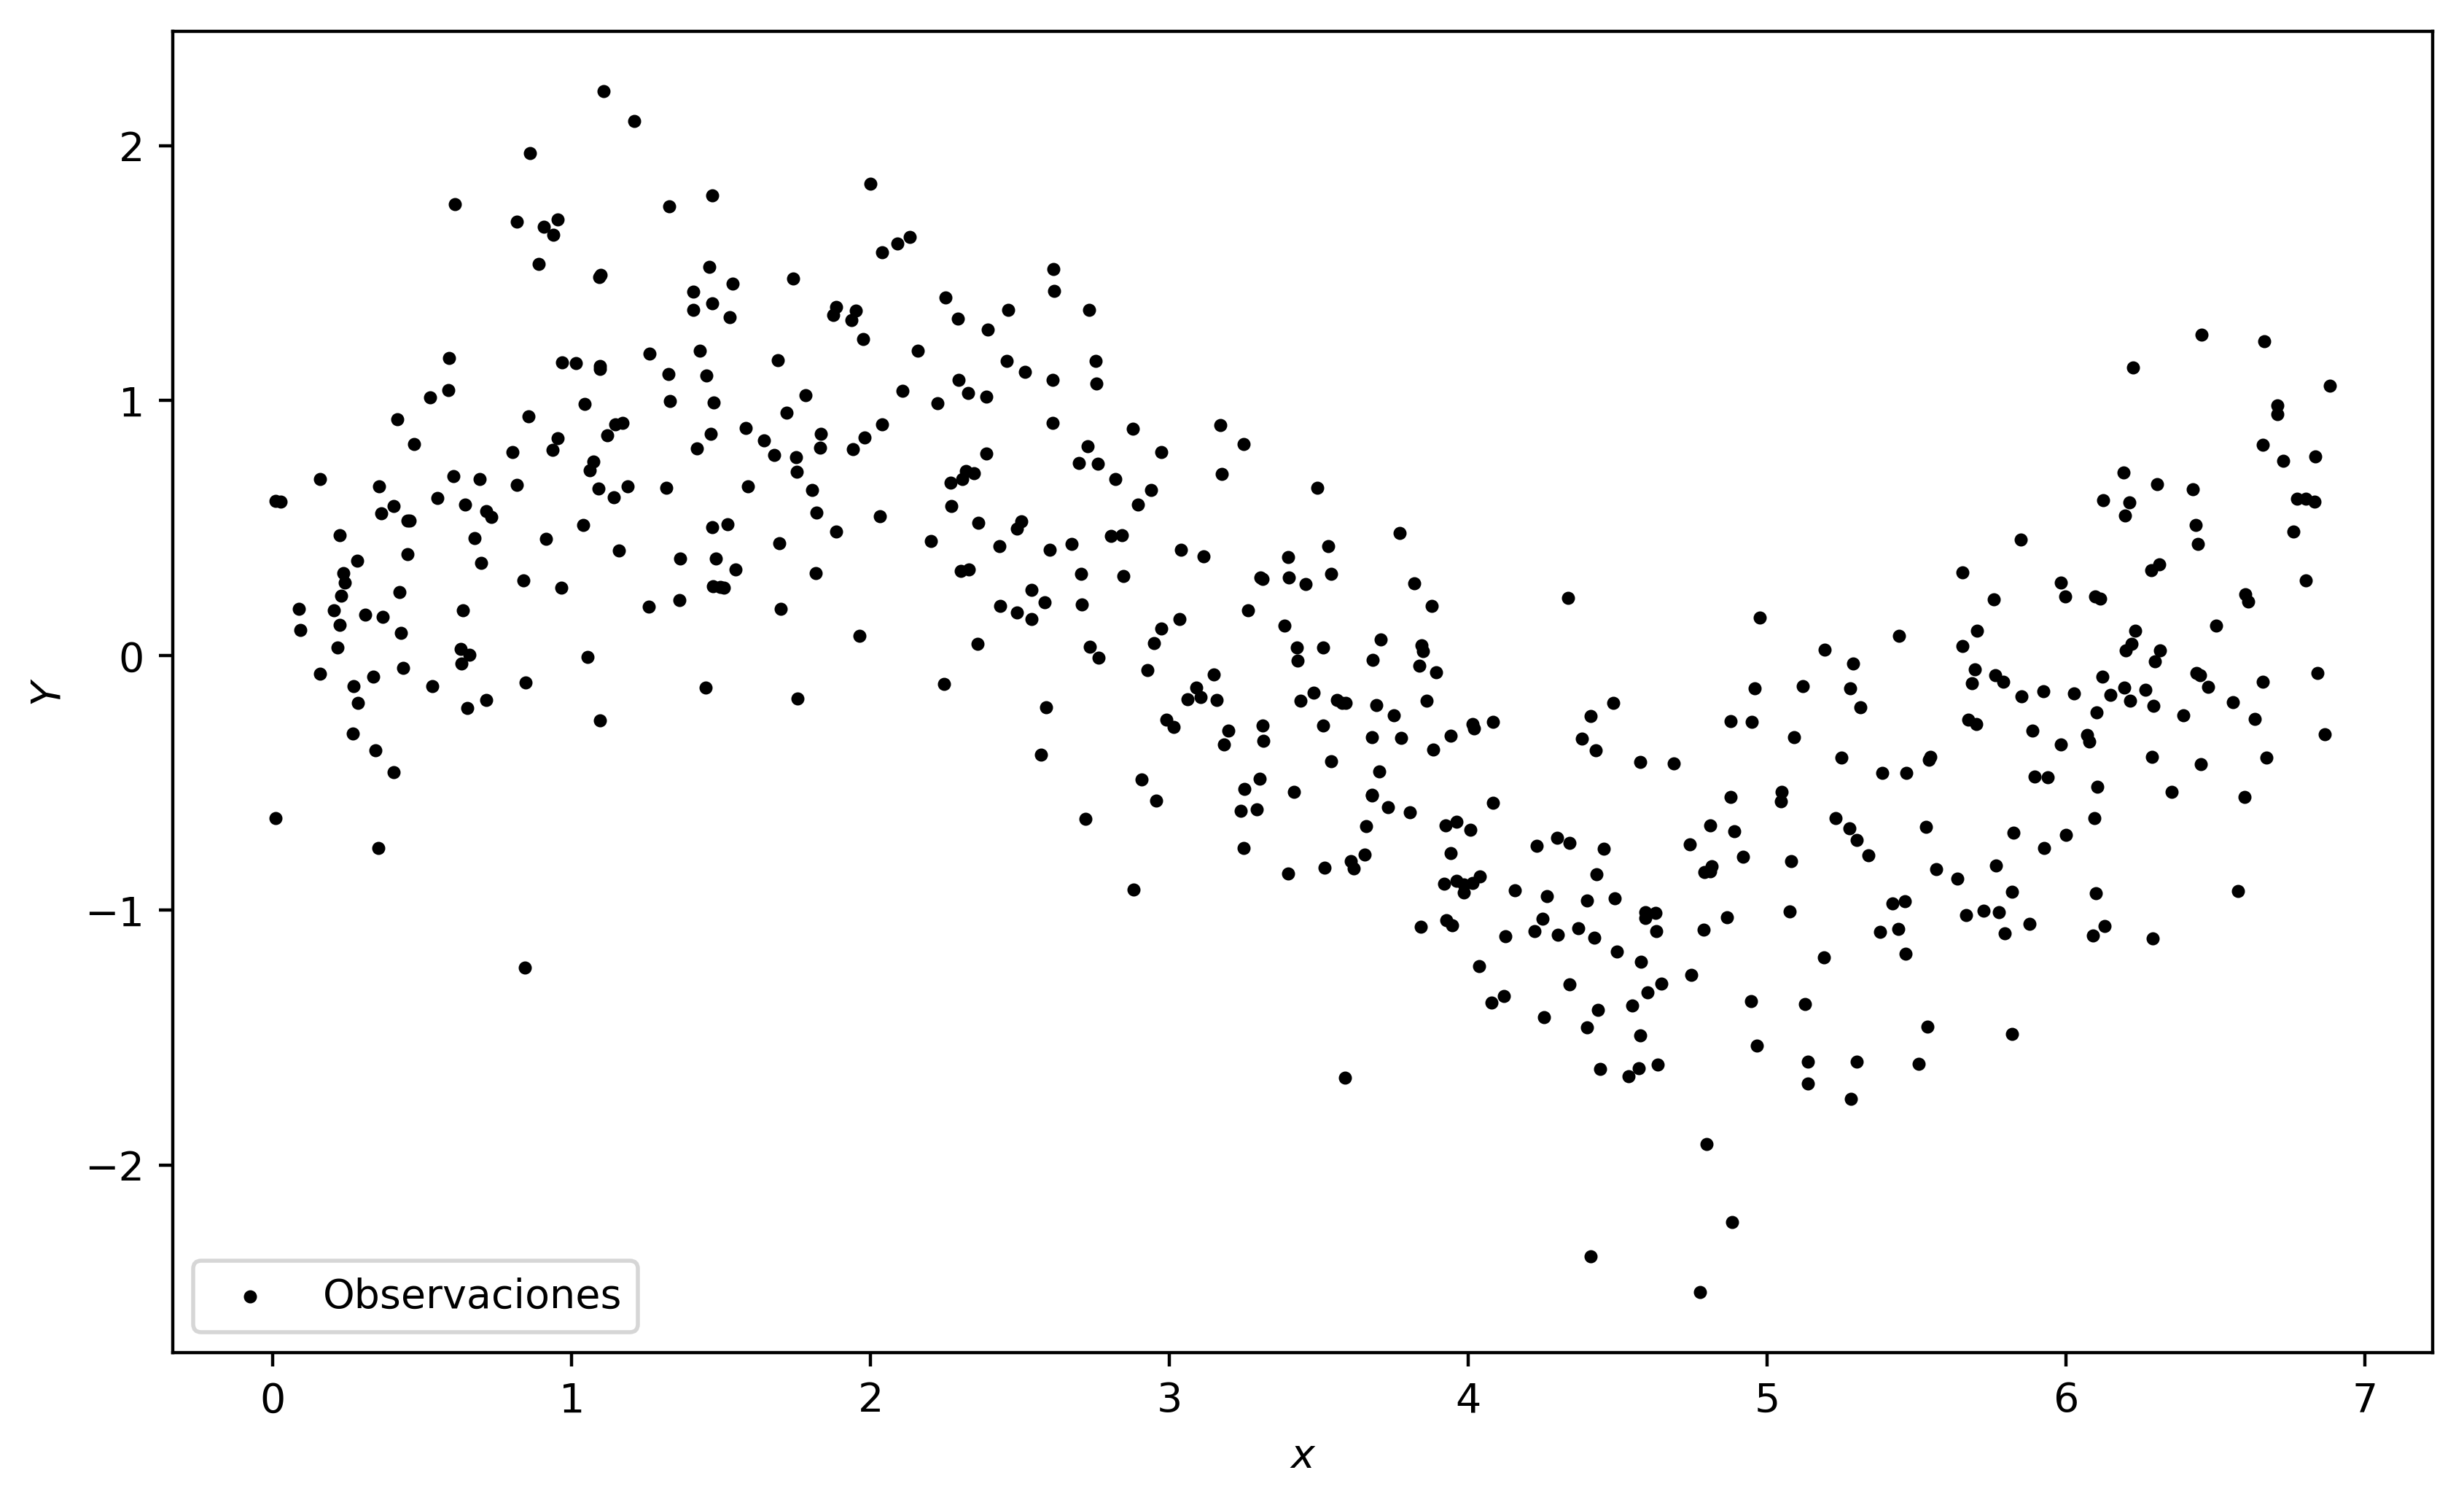
\includegraphics[scale=0.5]{regresion}

\end{frame}
\begin{frame}
\frametitle{Introducción}
\center
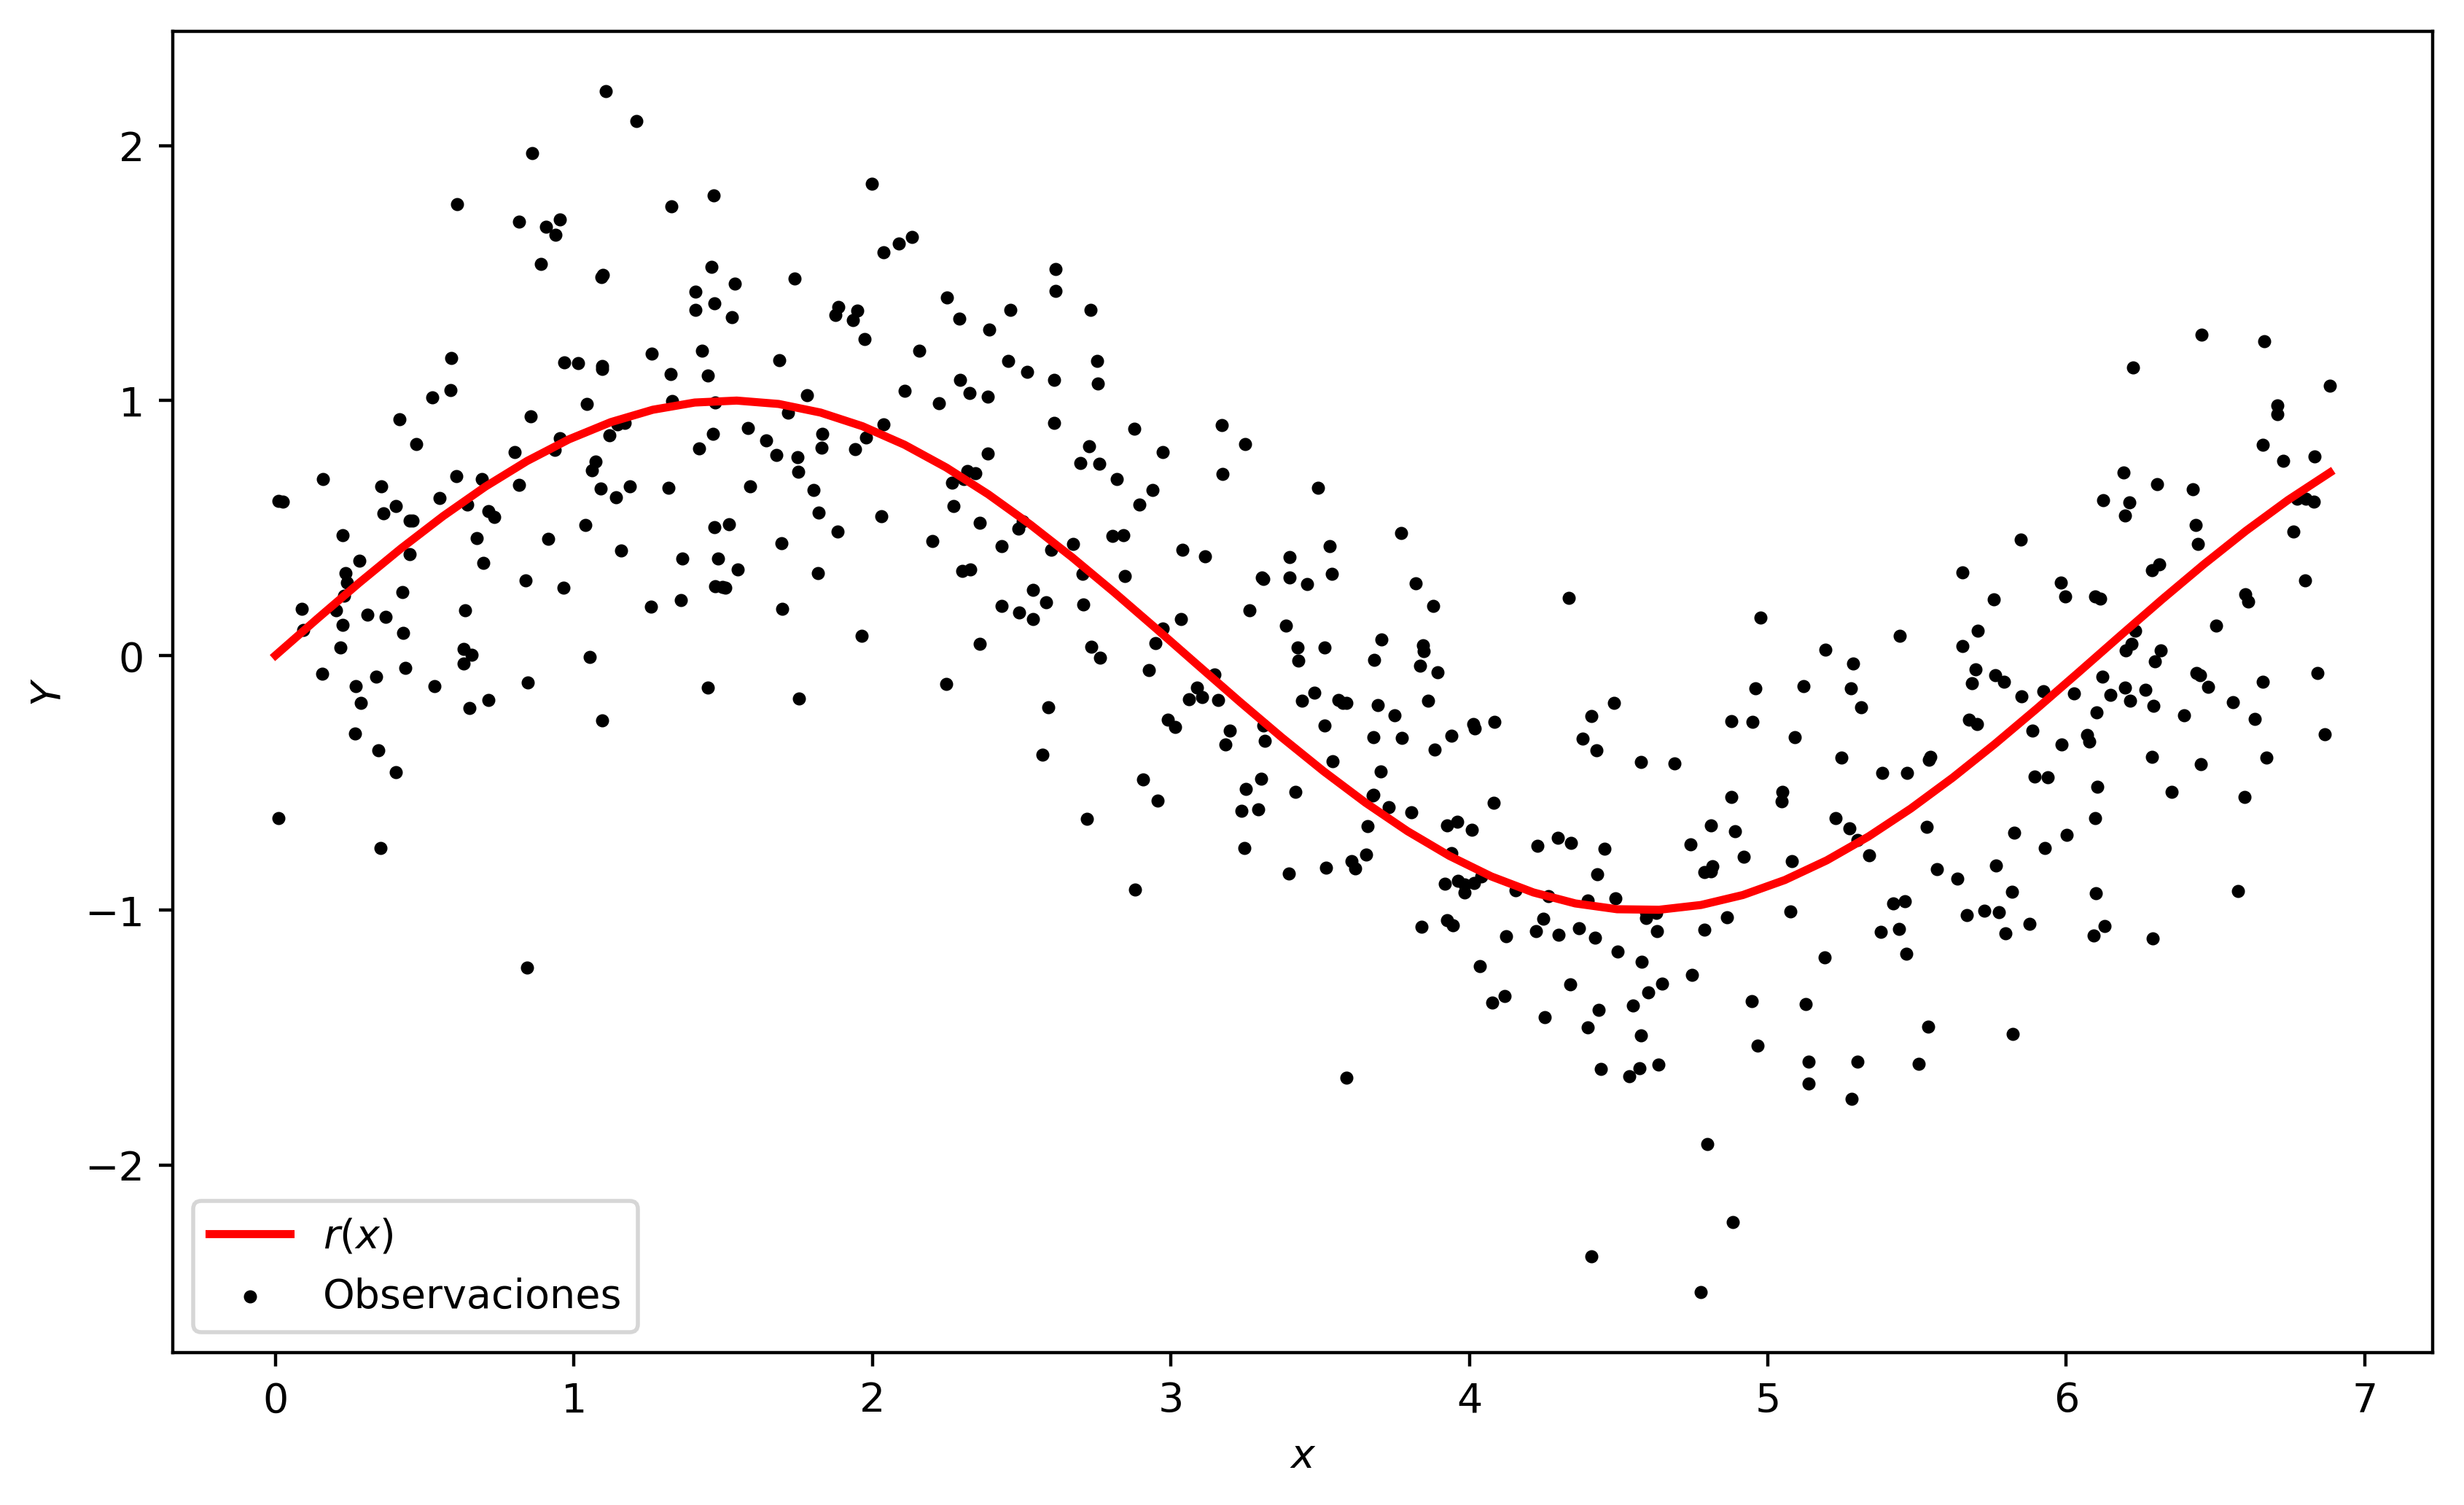
\includegraphics[scale=0.5]{regresion1}

\end{frame}
\begin{frame}
\frametitle{Introducción}
\center
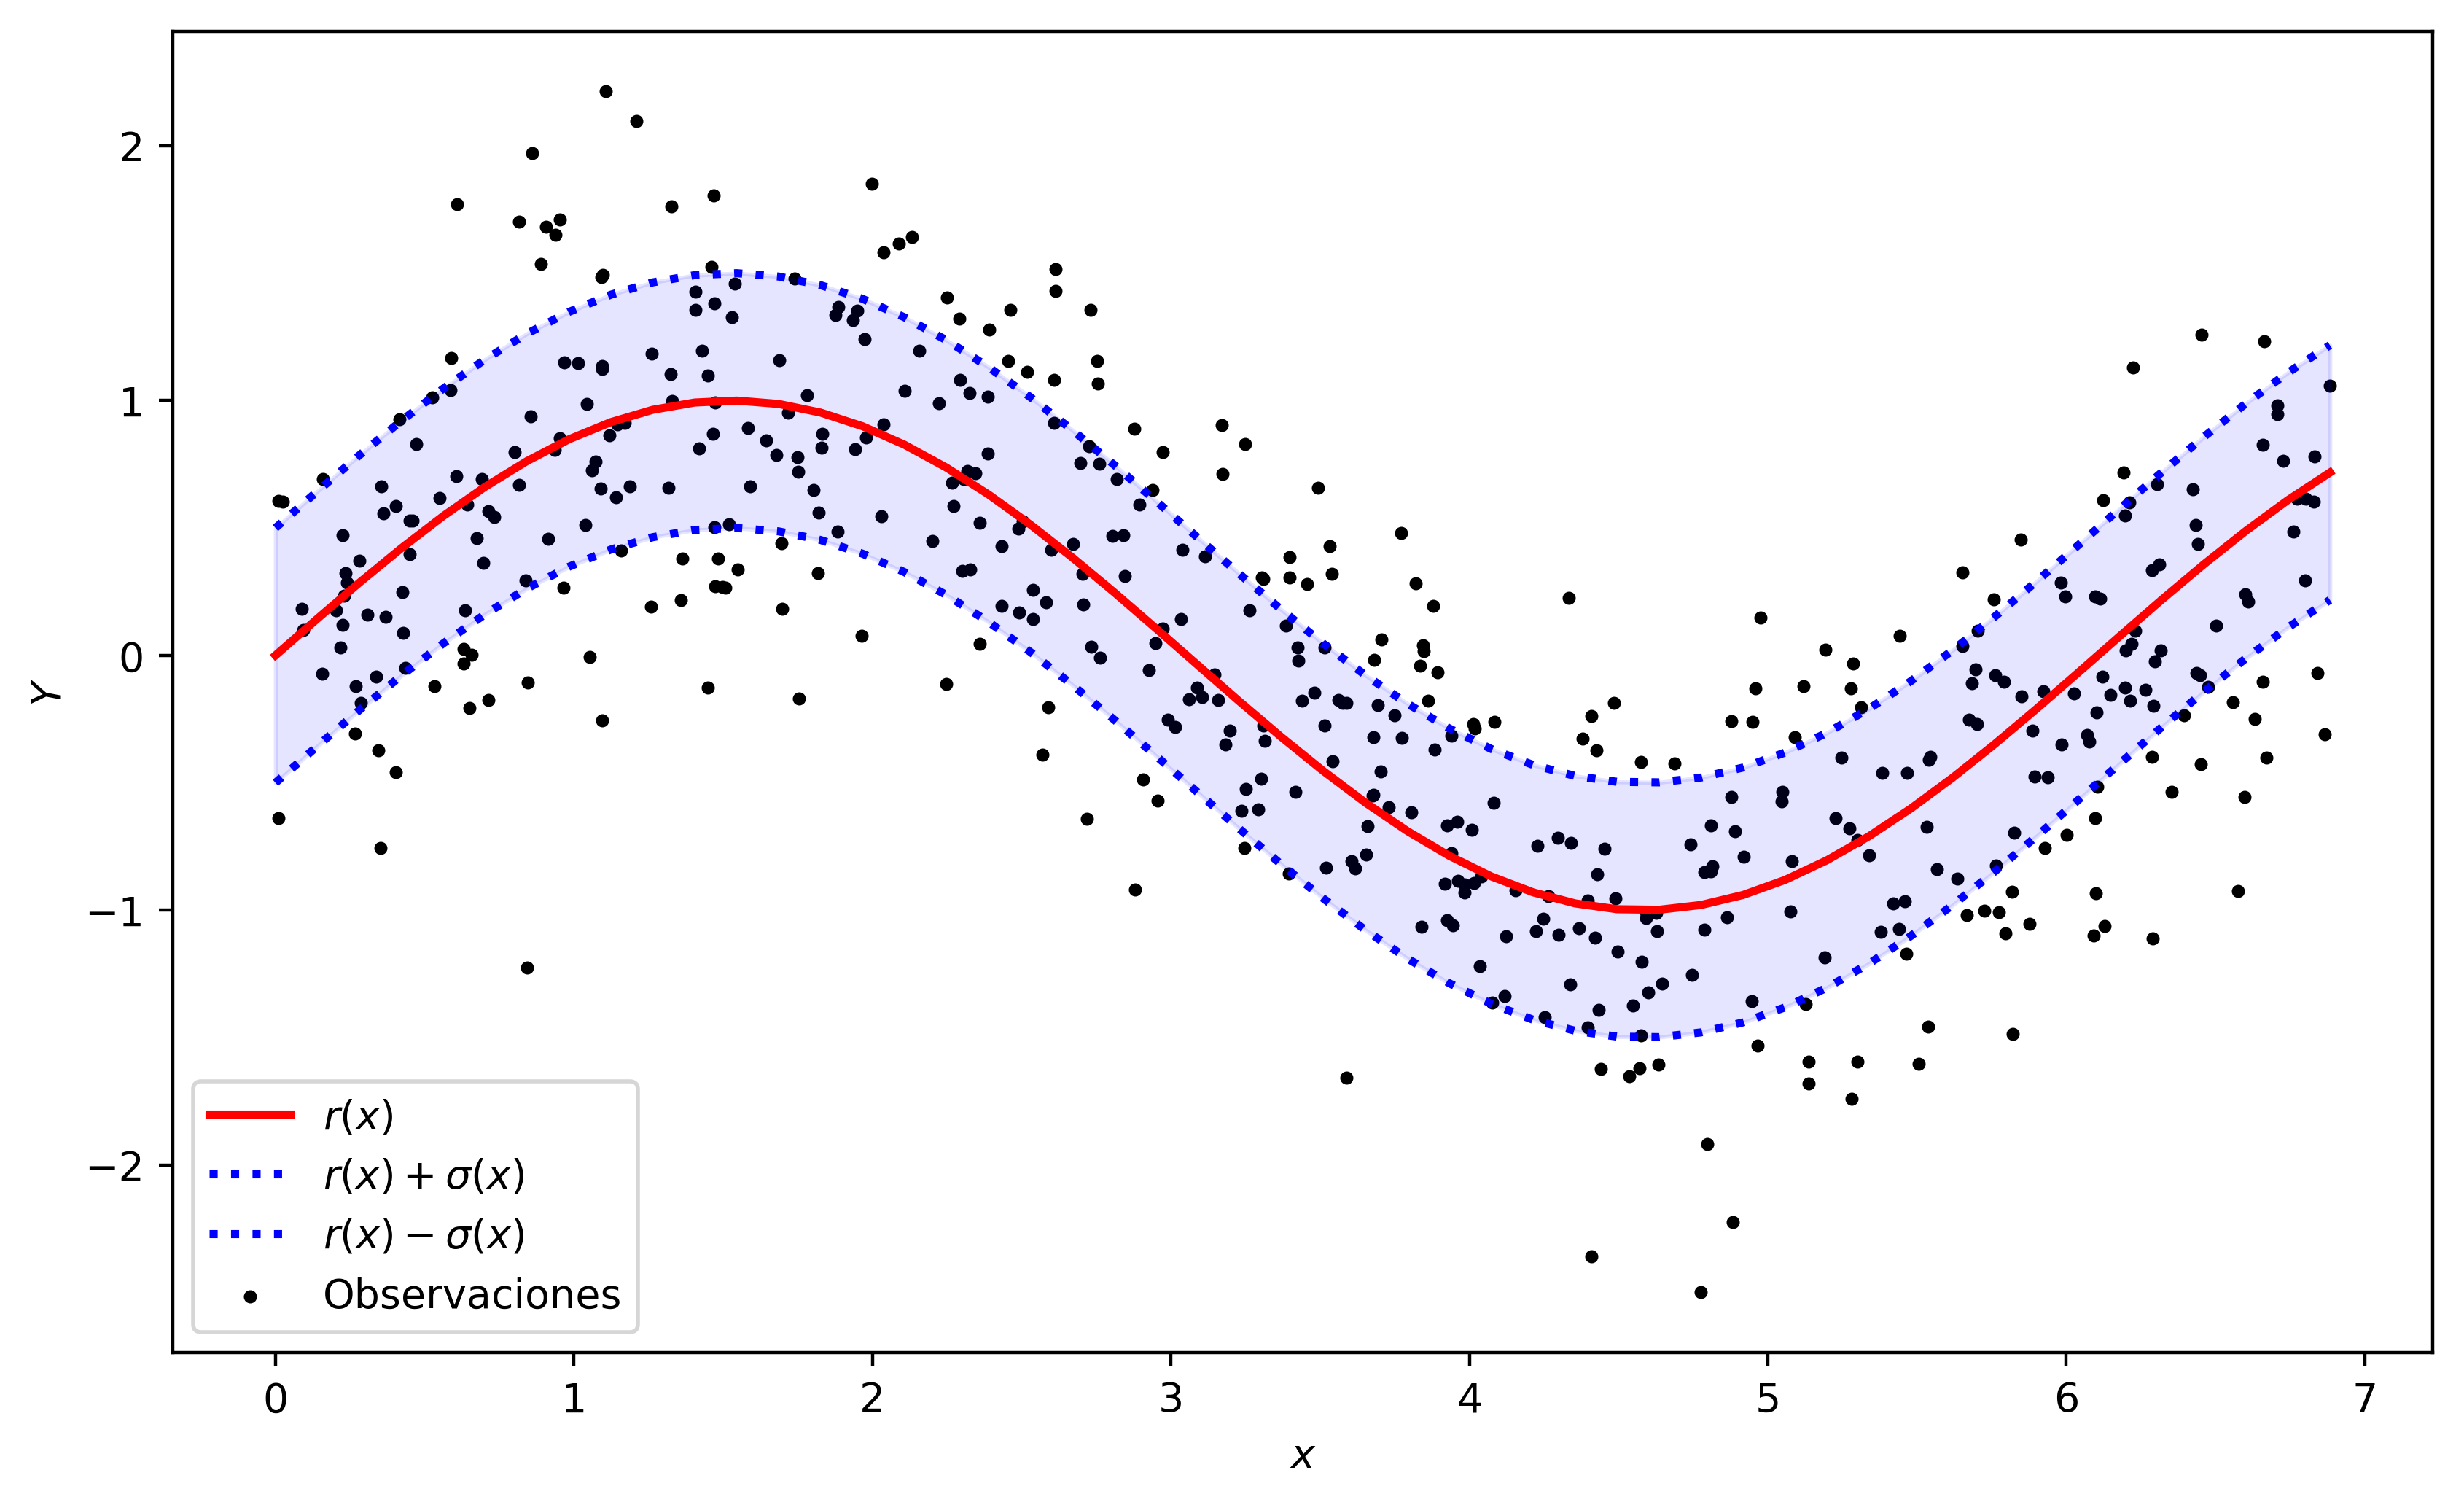
\includegraphics[scale=0.5]{regresion2}

\end{frame}

\begin{frame}
\frametitle{Regresores Lineales}
\section{Regresores Lineales}
Los tipos de funciones de regresores que veremos son \textbf{regresores lineales}
\begin{block}{Definición}
Un estimador $\hat{r}_n$ de $r$ es un \textbf{regreso lineal} sí para cada $x$ existe un vector $\ell(x)=(\ell_1(x),\ell_2(x),...,\ell_n(x))^{T}$ tal que $$\hat{r}_n(x)=\sum_{i=1}^{n}\ell_i(x)Y_i$$

\end{block}
\end{frame}
\begin{frame}
\frametitle{Regresores Lineales}
Se define el vector de los \textbf{valores ajustados} como $$\textbf{r}=(\hat{r}_n(x_1),...,\hat{r}_n(x_n))^{T}$$
de esta forma si definimos $Y=(Y_1,...,Y_n)^{T}$ podemos escribir $\textbf{r}$ como 
$$\textbf{r} = LY$$
donde $L$ es una matriz de $n\times n$ con valores $L_{ij}=\ell_j(x_i)$.
\end{frame}

\begin{frame}
\frametitle{Regresores Lineales}

\textbf{Ejemplo 1 }
Dividimos nuestro intervalo $(a,b)$ en m bins del mismo tamaño lo cuales denotamos como $B_1,...,B_m$, definimos $\hat{r}_n(x)$ como 
$$\hat{r}_n(x)=\frac{1}{k_j}\sum_{i:x_i\in B_j}^{n}Y_i$$
Donde $k_j$ es la cantidad de observaciones en $B_j$
\end{frame}

\begin{frame}
\frametitle{Regresores Lineales}
\center
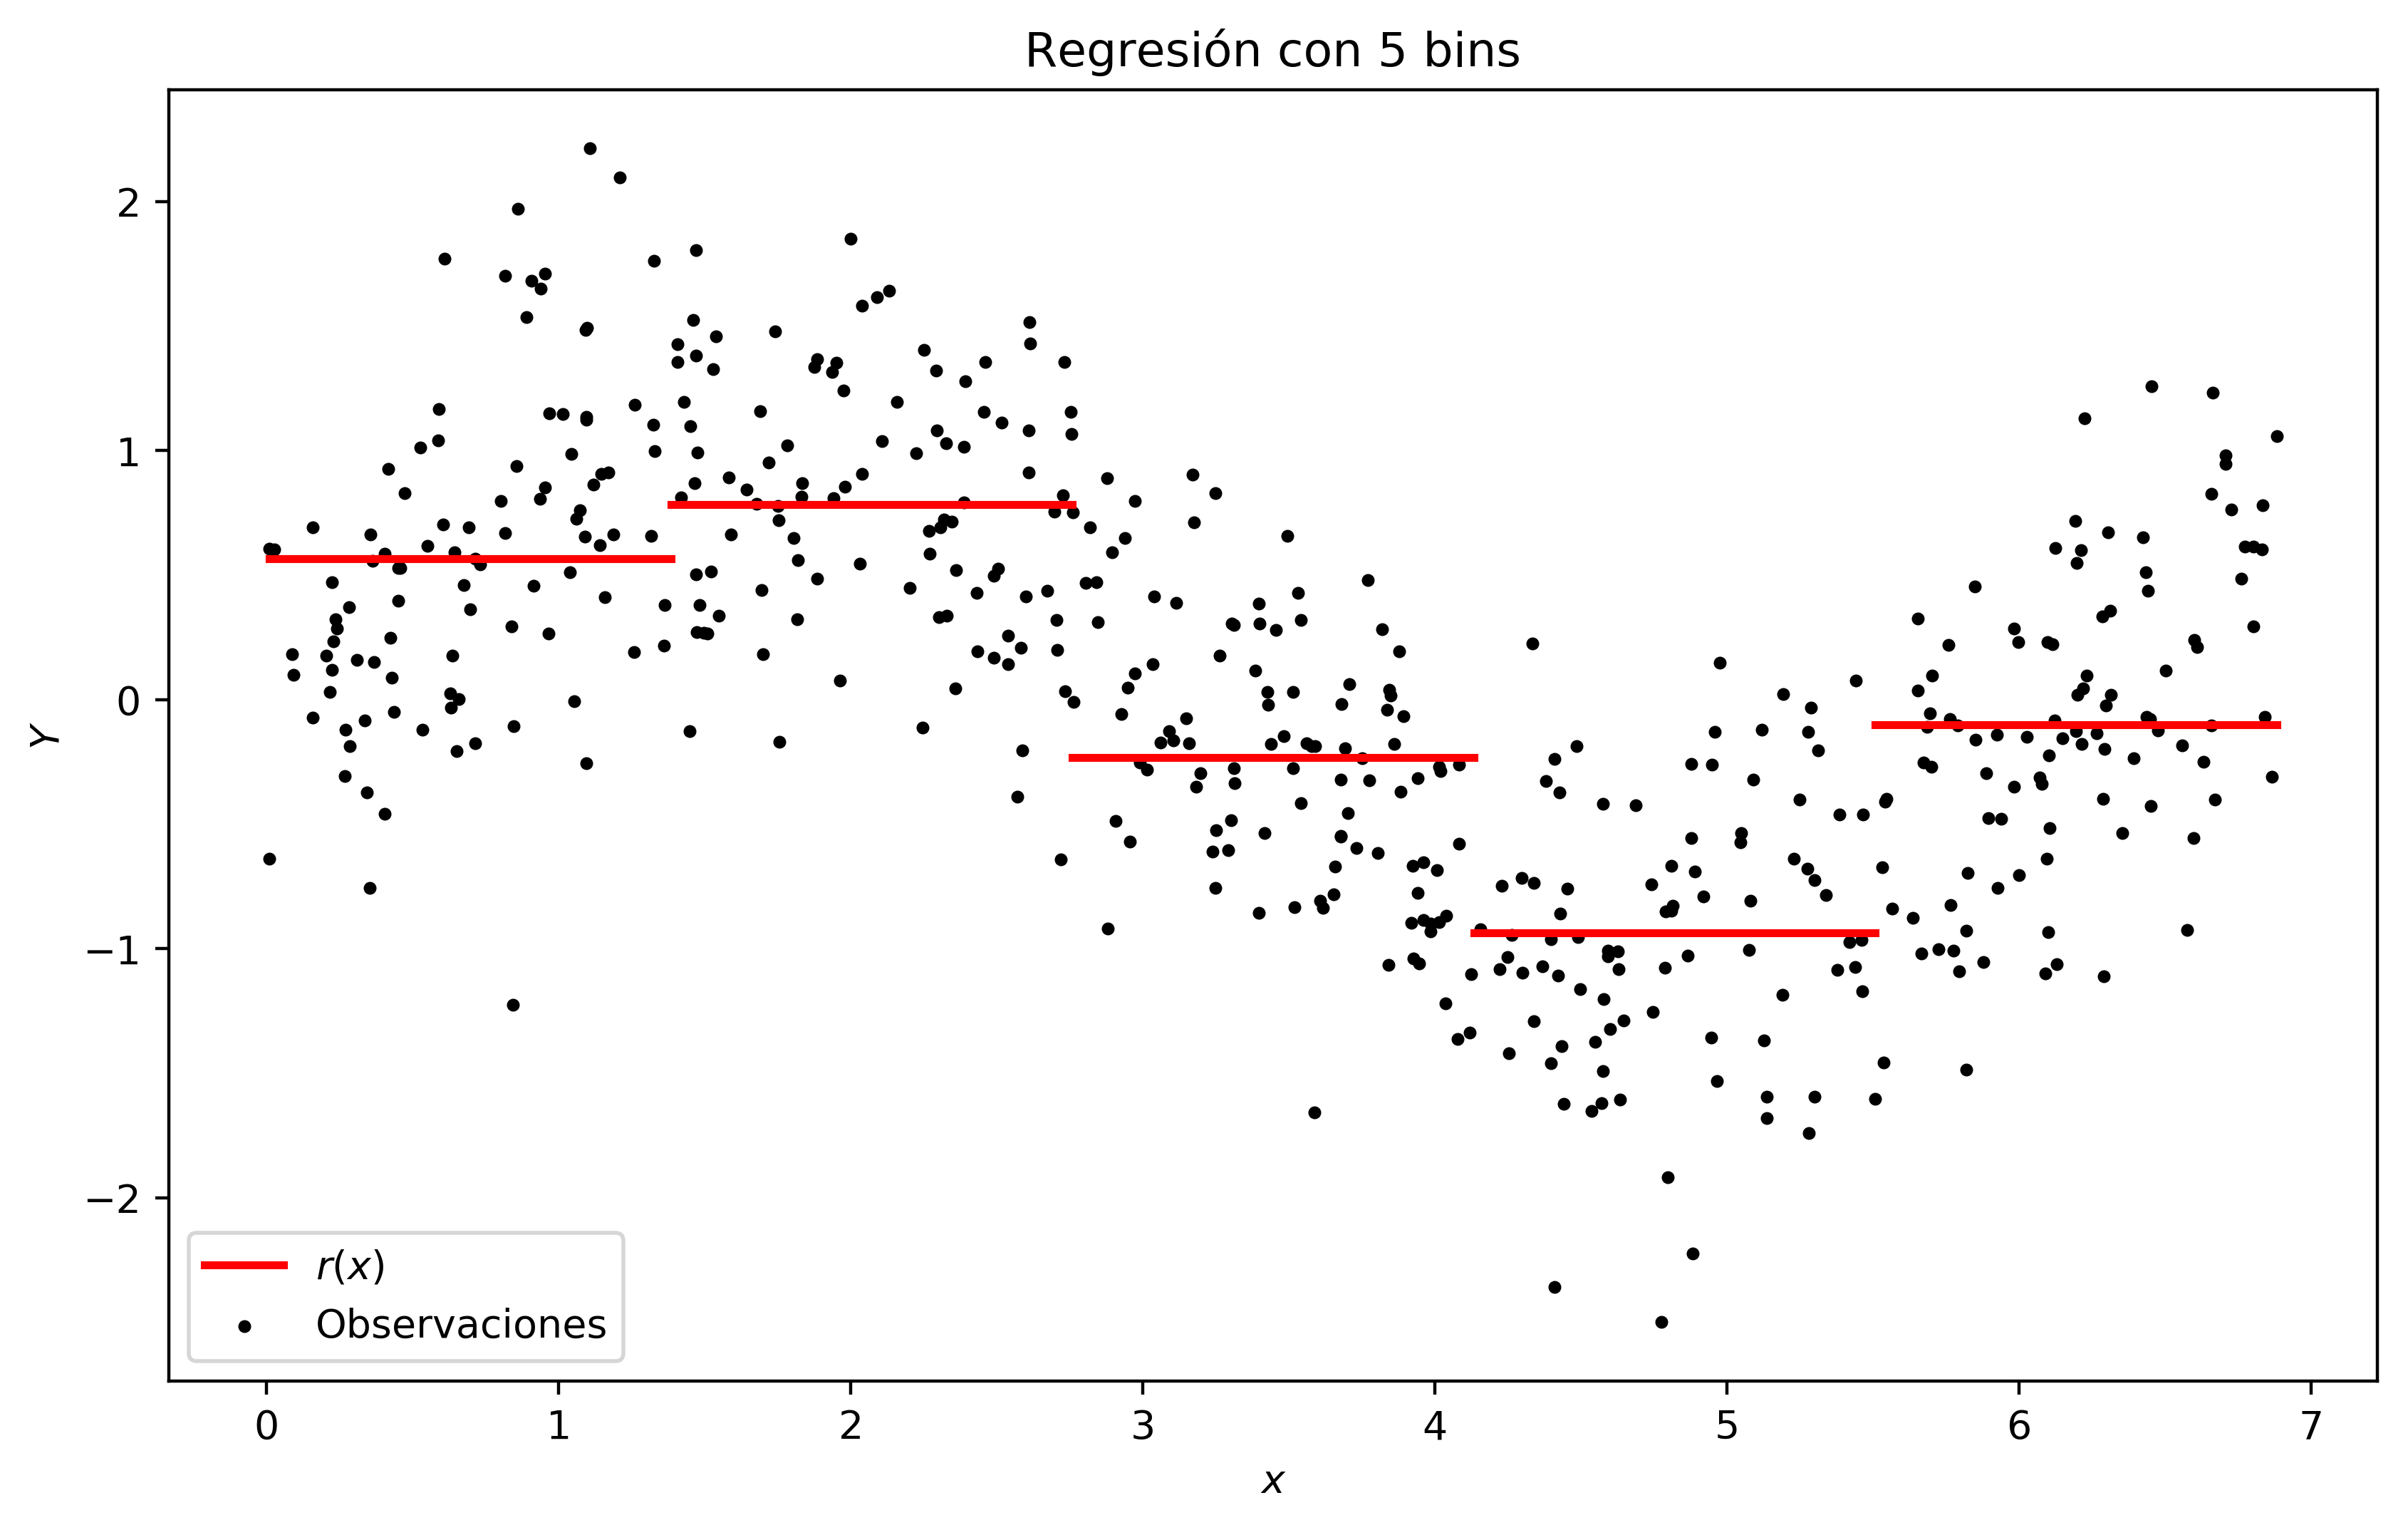
\includegraphics[scale=0.5]{regresion3}

\end{frame}
\begin{frame}
\frametitle{Regresores Lineales}
\center
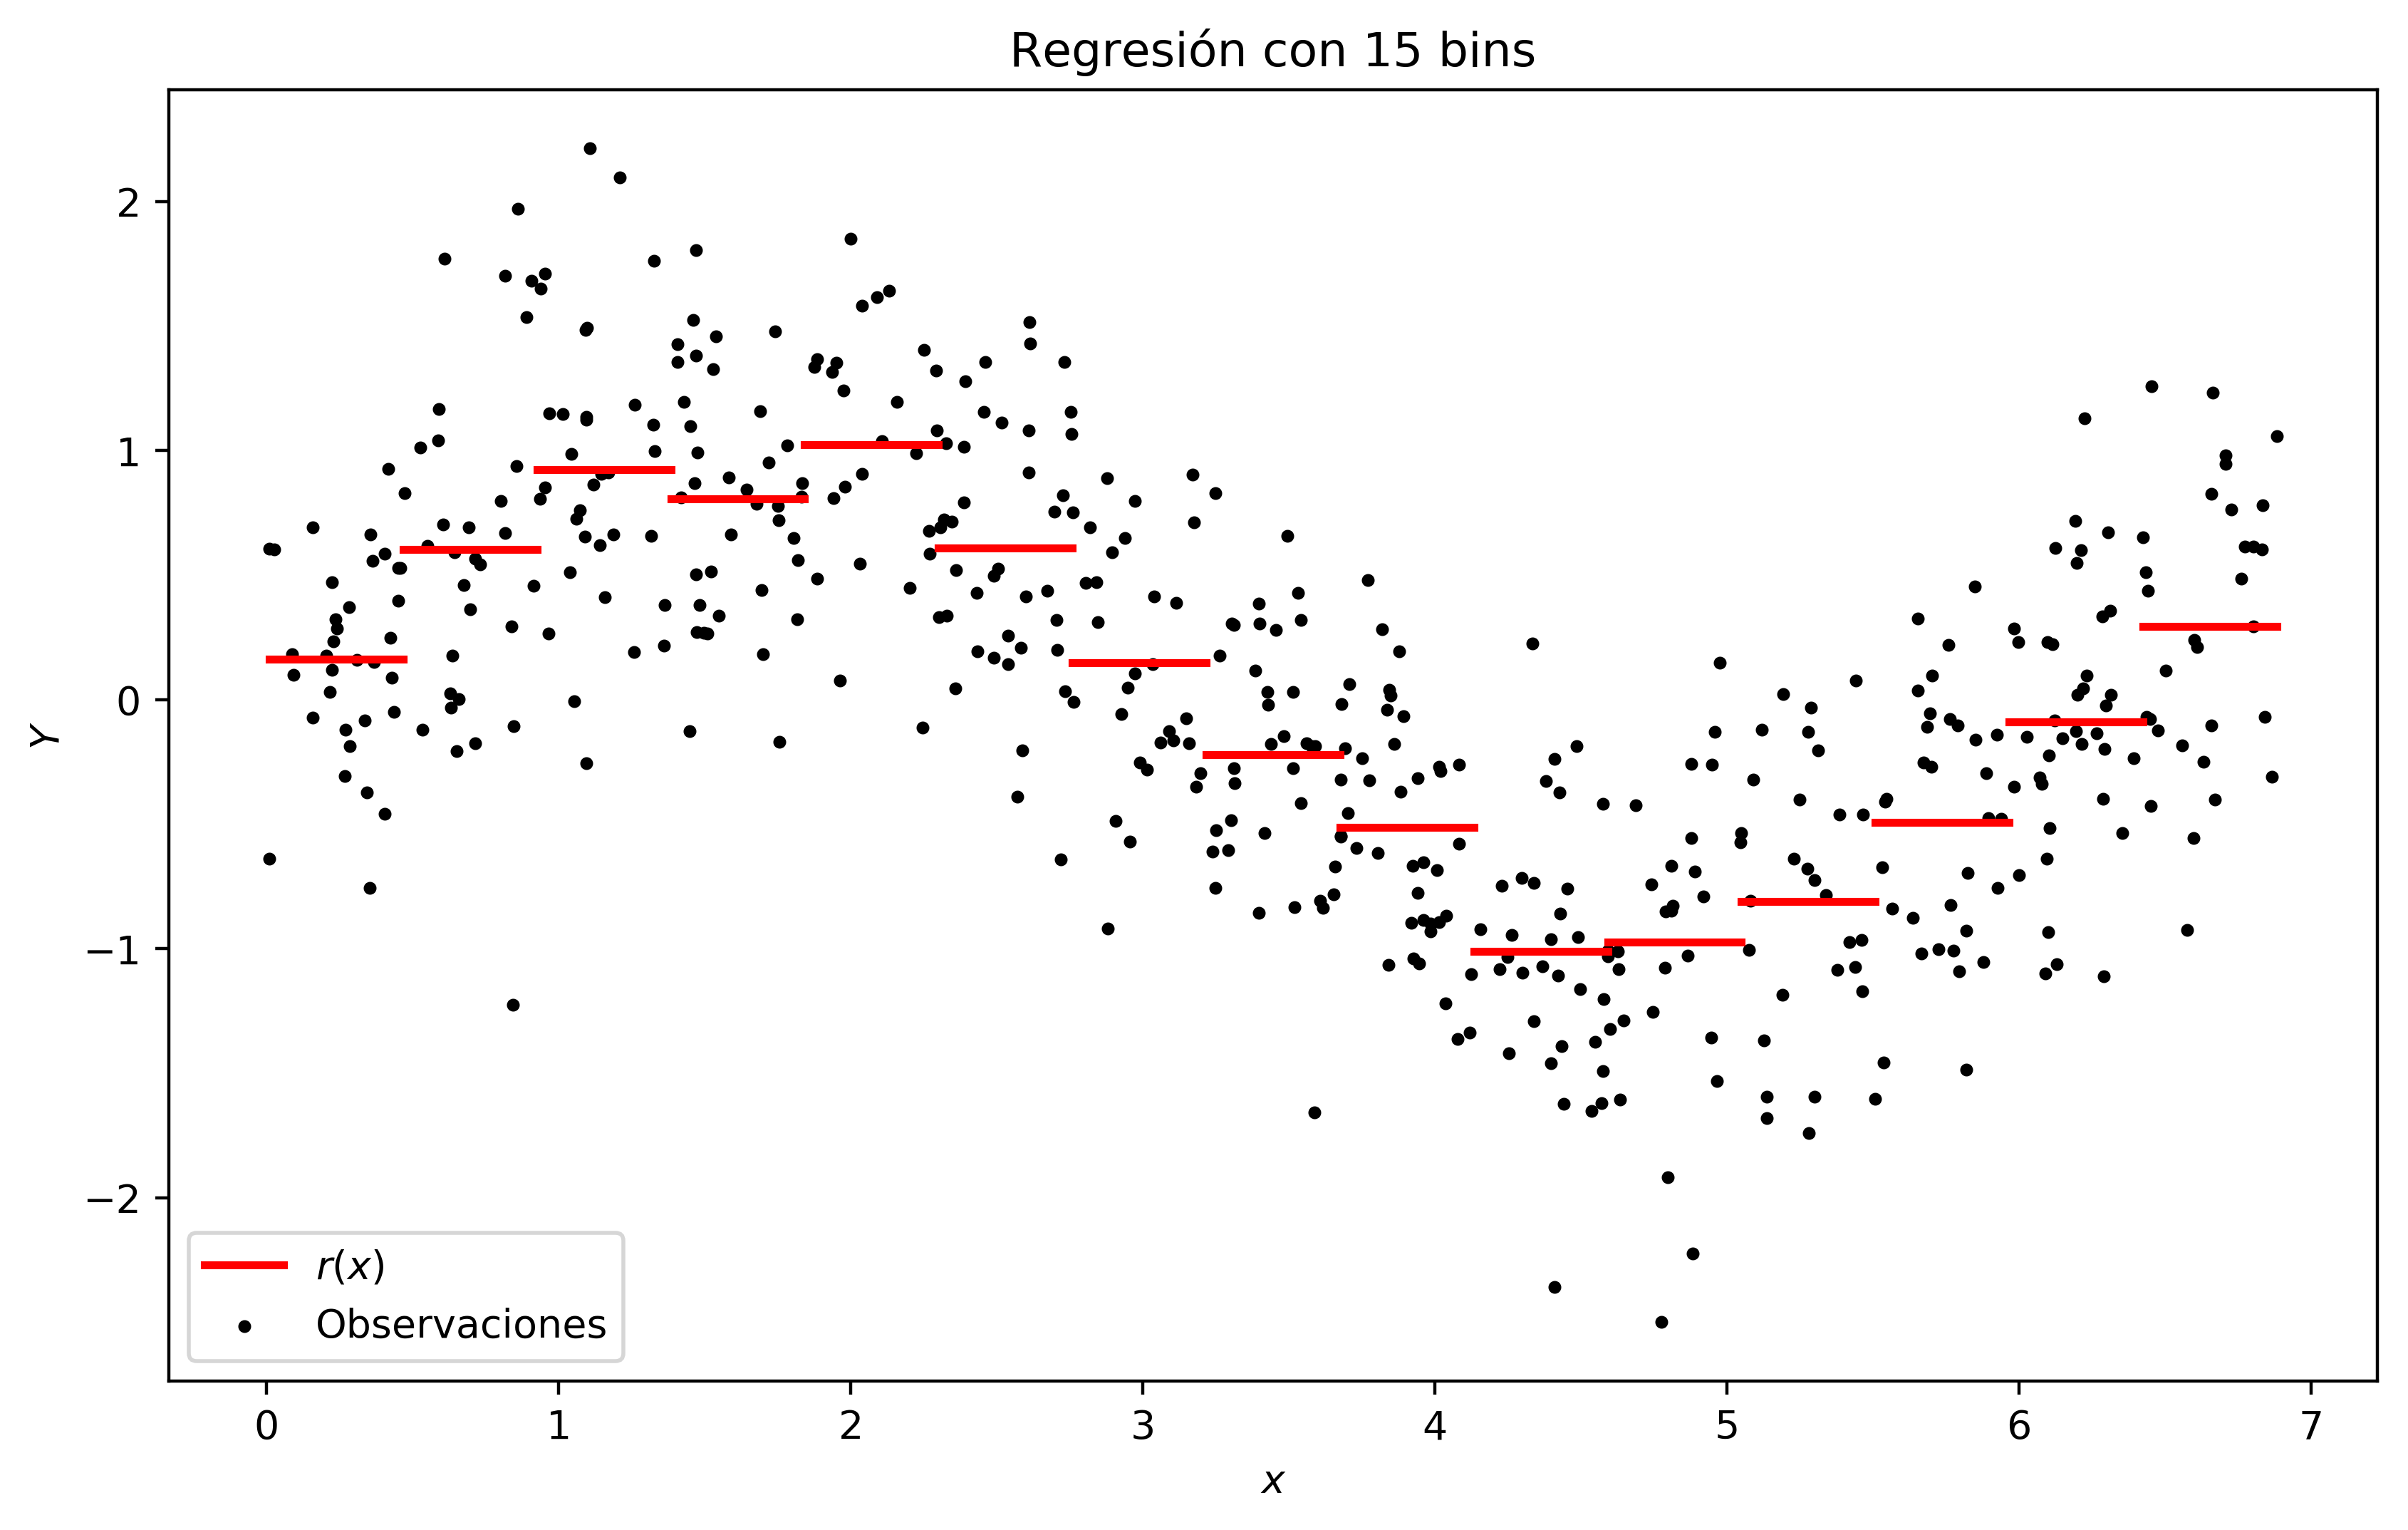
\includegraphics[scale=0.5]{regresion4}

\end{frame}


\begin{frame}
\frametitle{Regresores Lineales}

\textbf{Ejemplo 2}
Sea $h>0$ y $B_x=\{i:|x_i-x|\le h\}$, sea $n_x$ la cantidad de puntos que pertenecen a $B_x$, para cada $x$ tal que $n_x>0$ se define  


$$\hat{r}_n(x)=\frac{1}{n_x}\sum_{i\in B_x}^{n}Y_i$$
\end{frame}

\begin{frame}
\frametitle{Regresores Lineales}
\center
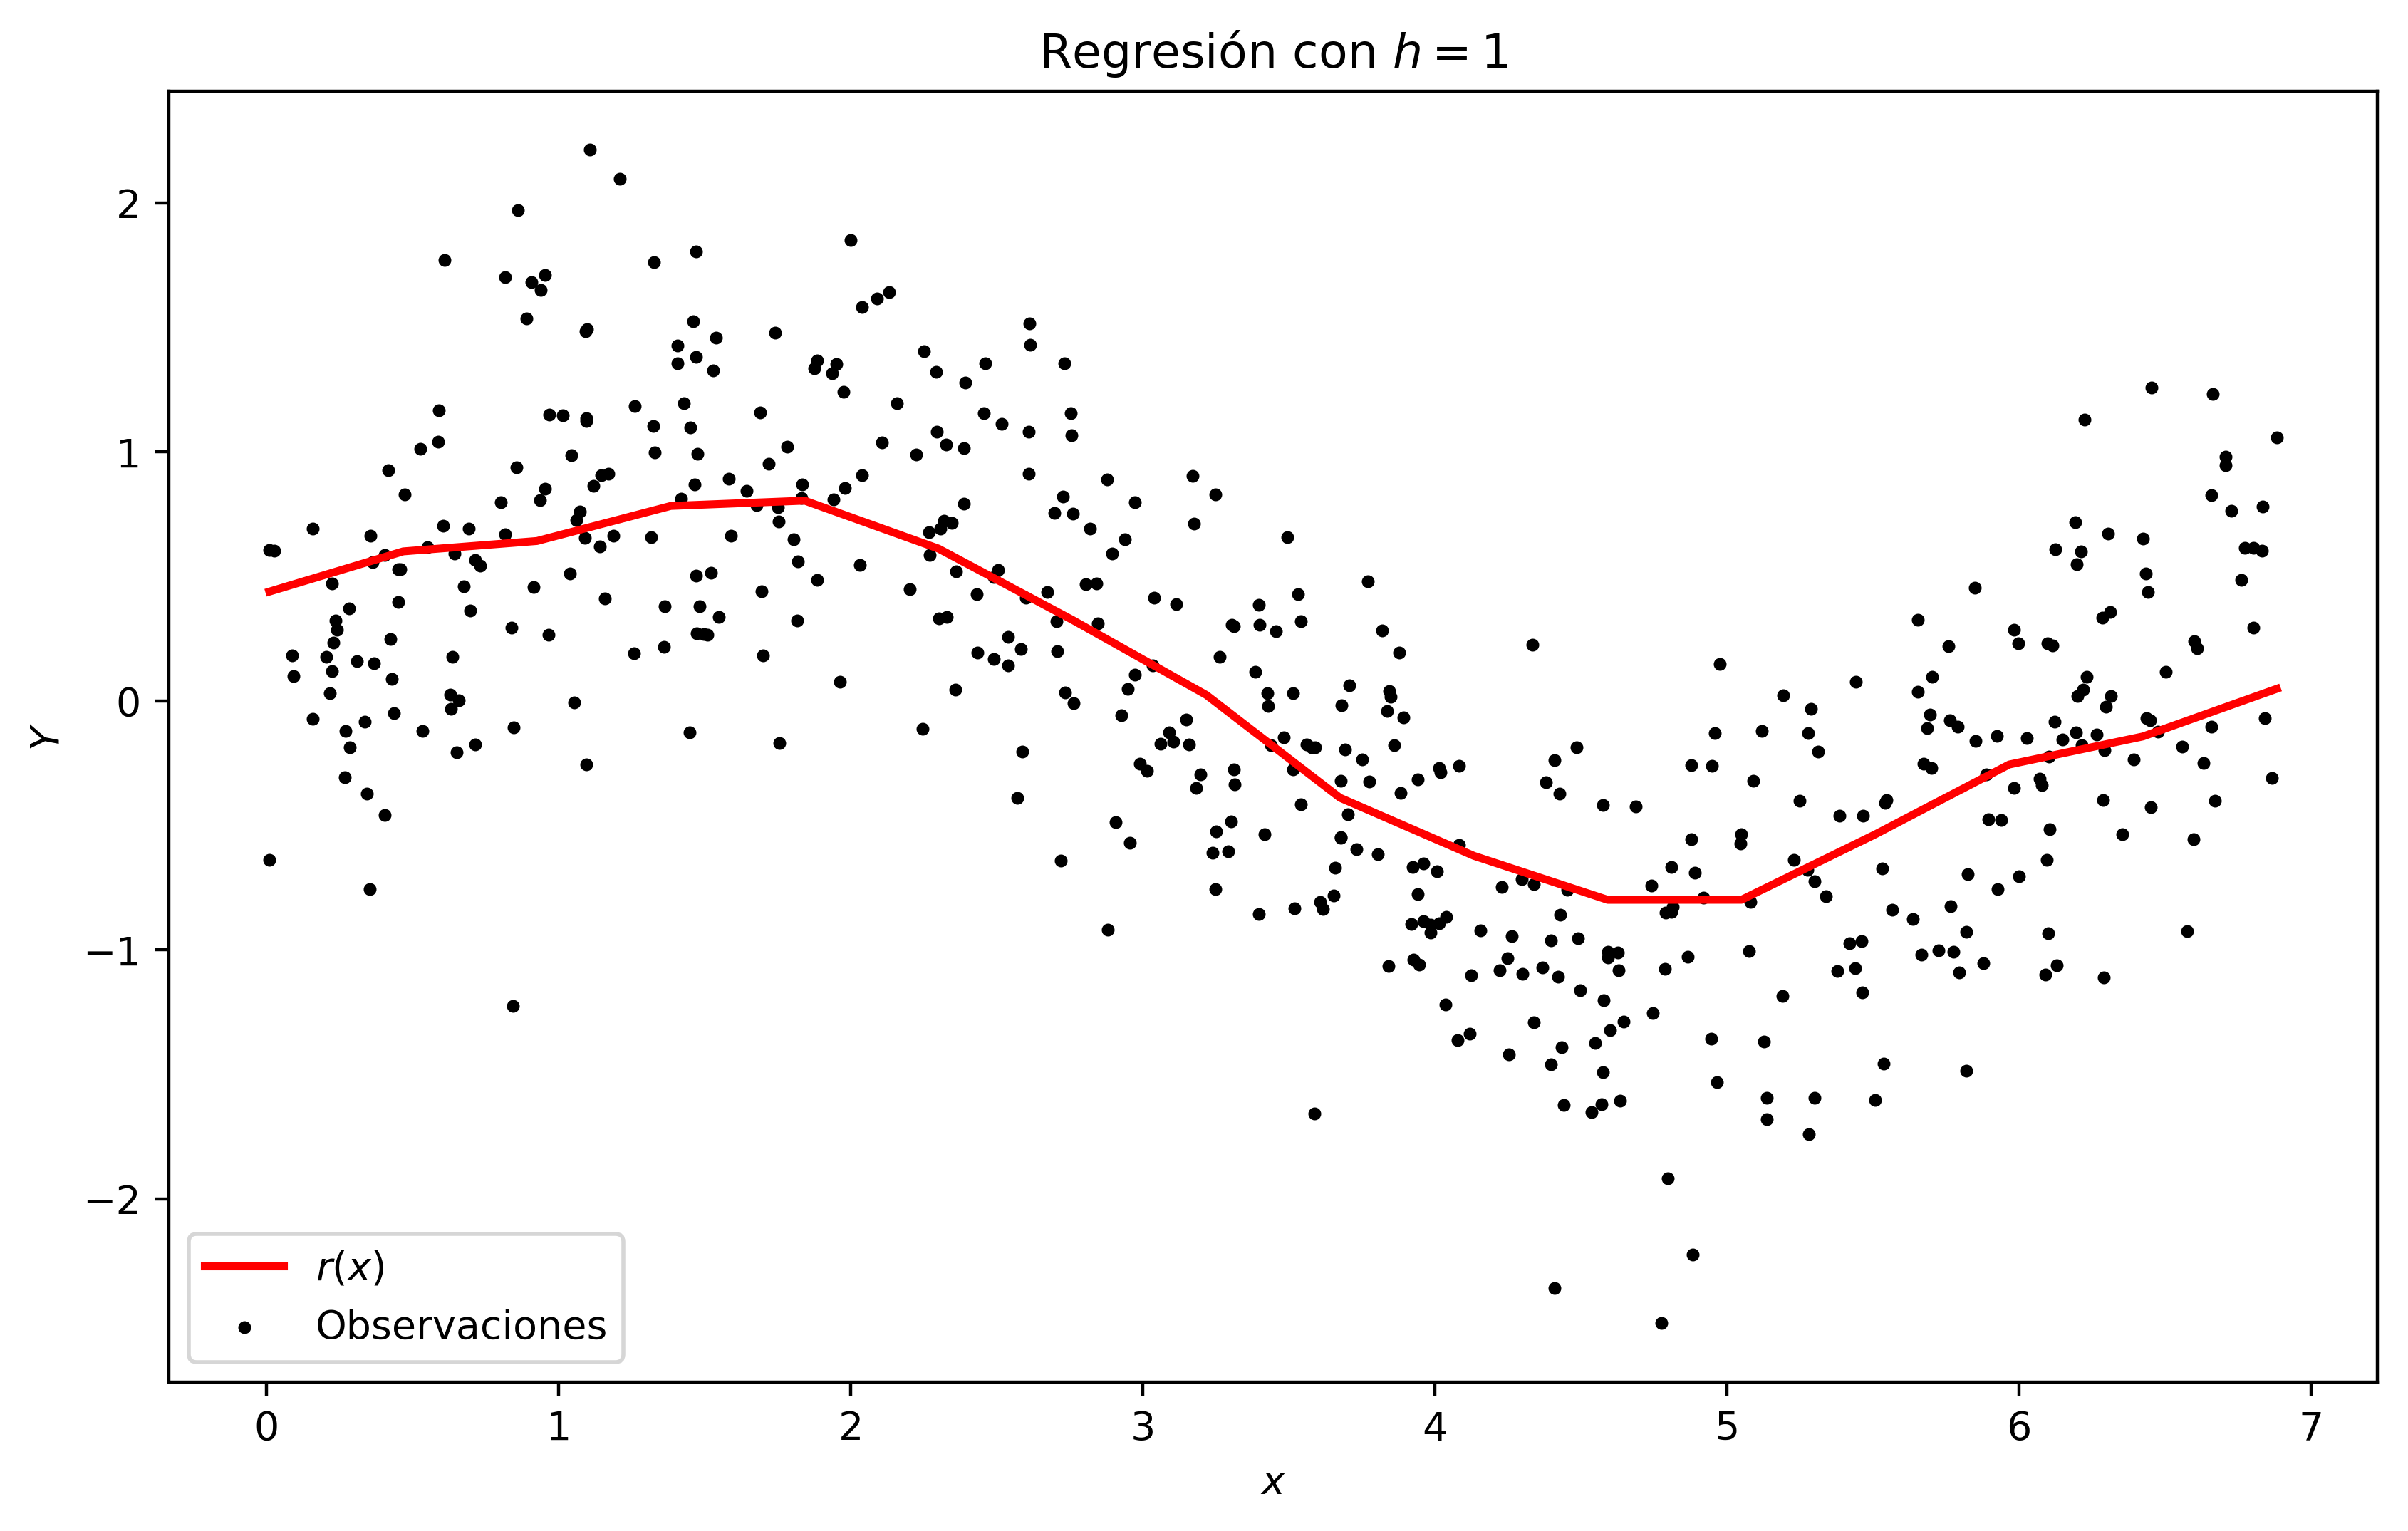
\includegraphics[scale=0.5]{regresion5}
\end{frame}
\begin{frame}
\frametitle{Regresores Lineales}
\center
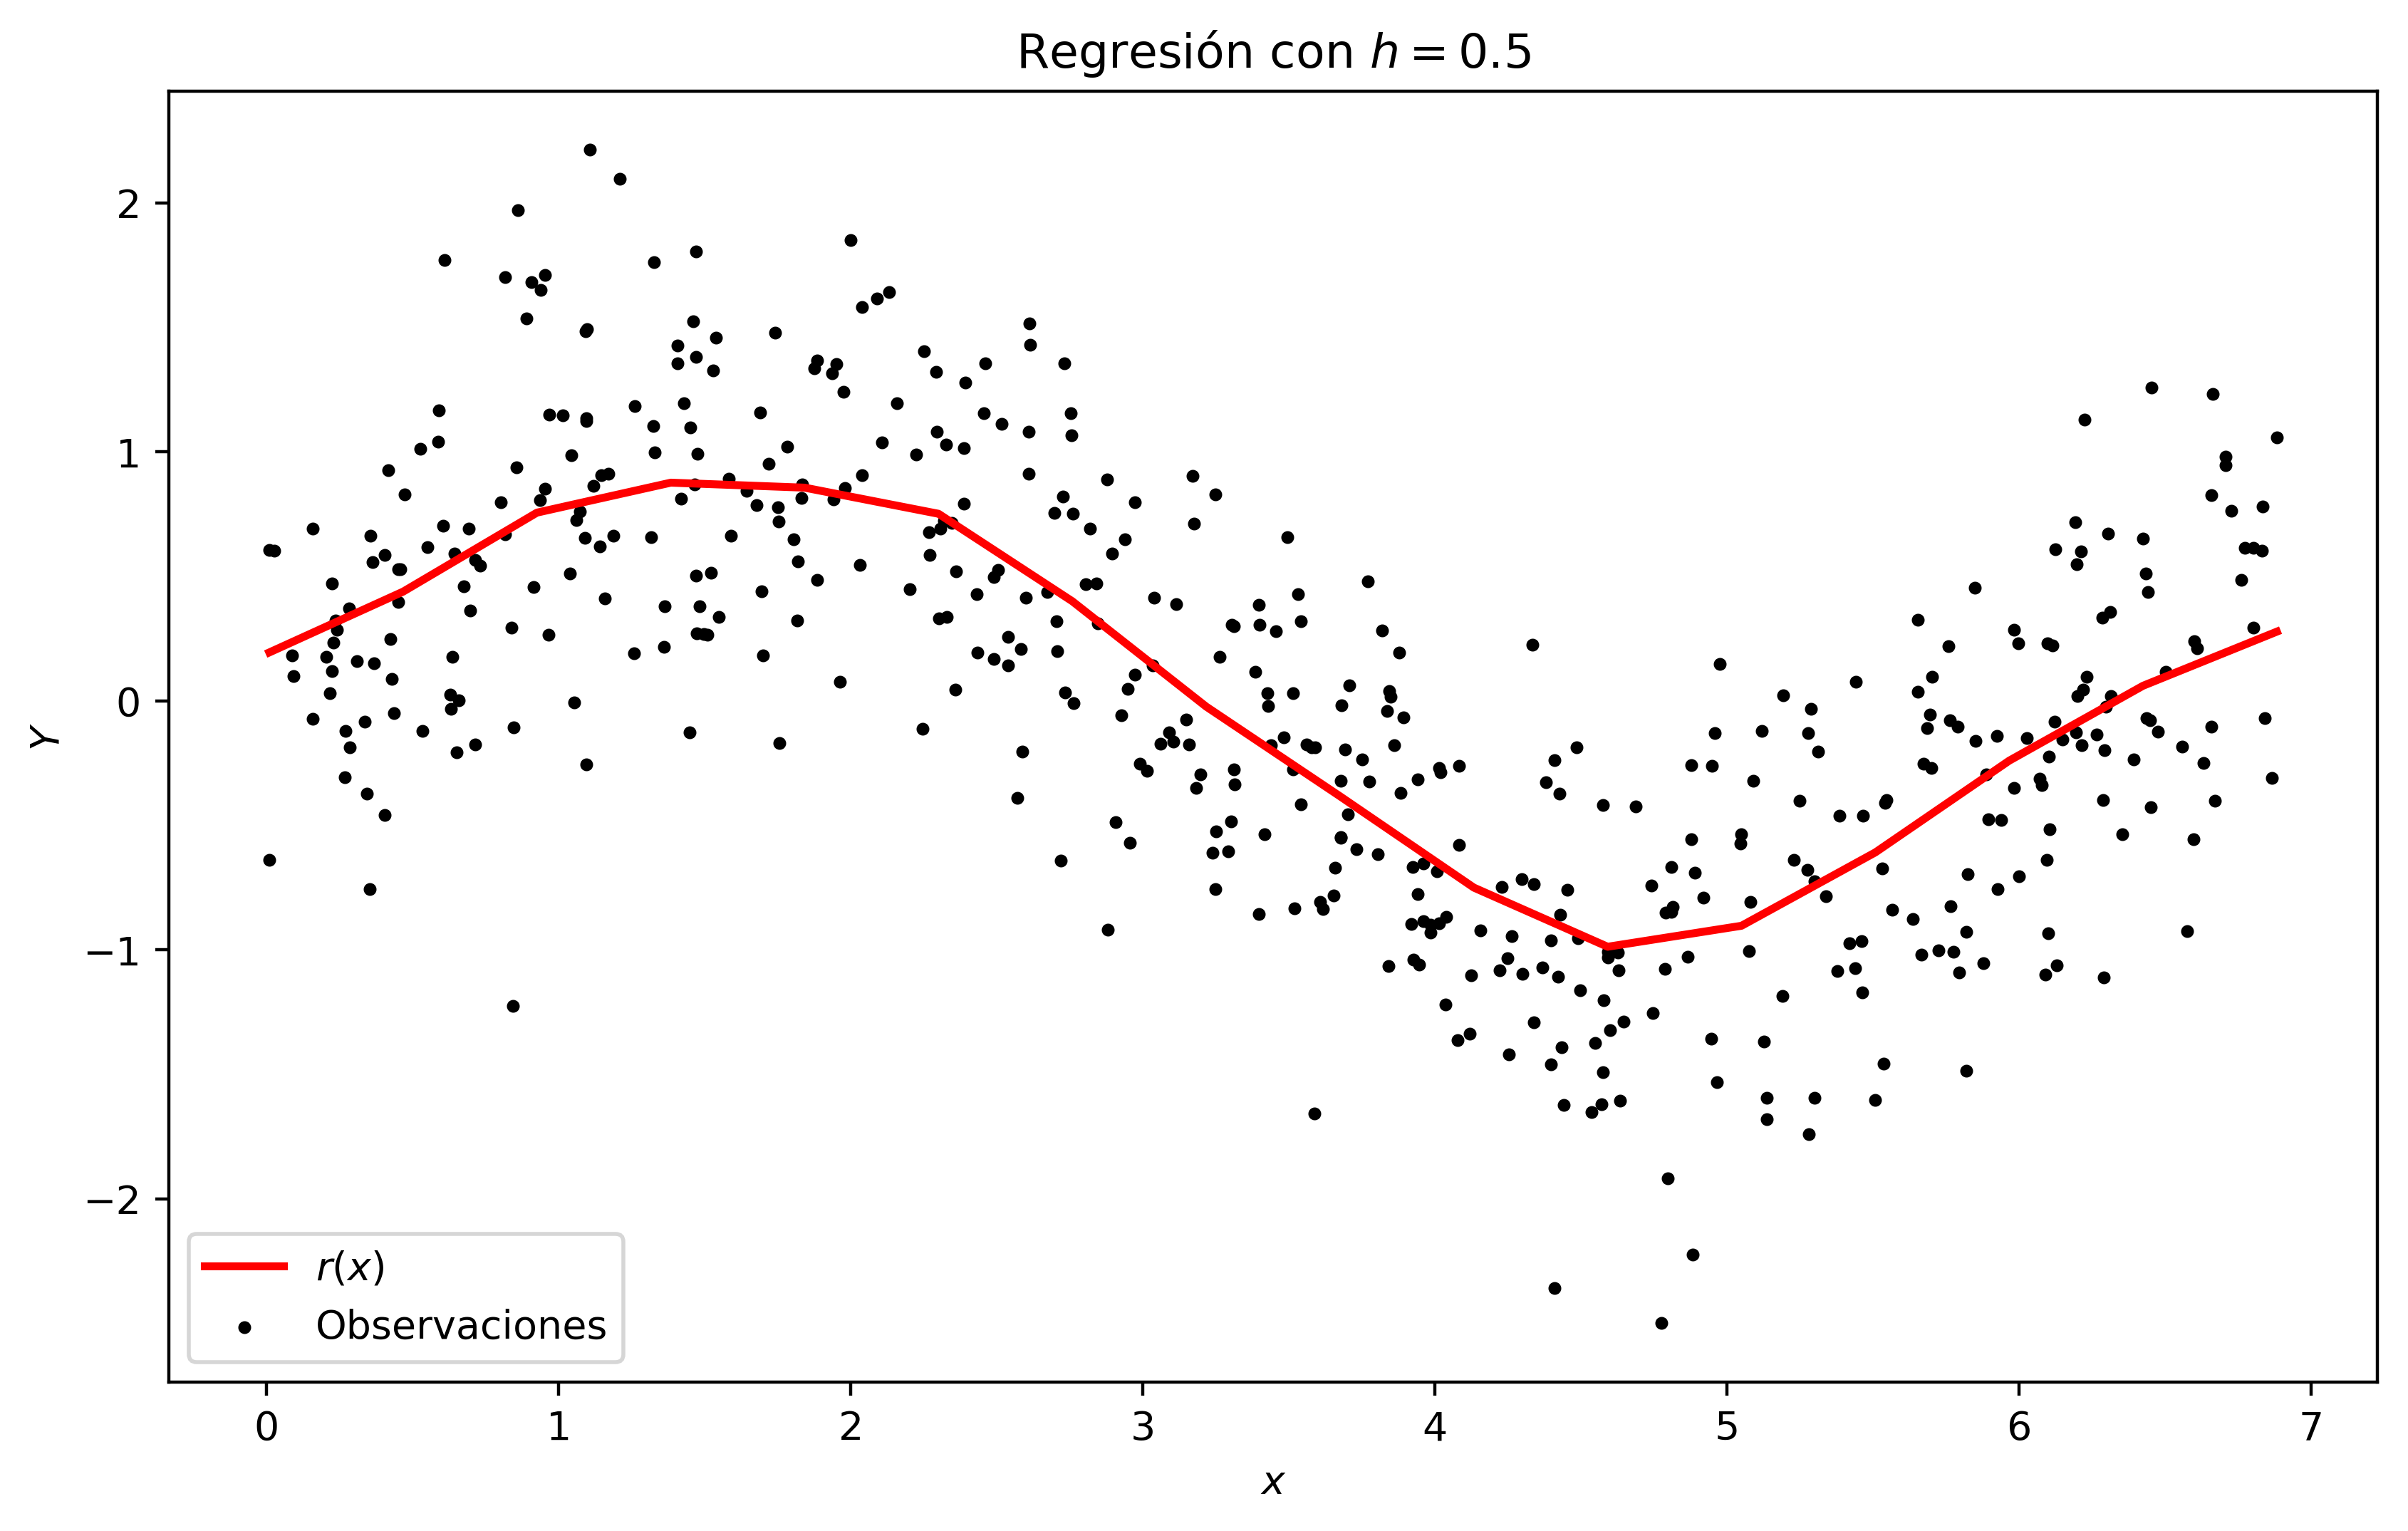
\includegraphics[scale=0.5]{regresion6}
\end{frame}
\begin{frame}
\frametitle{Regresores Lineales}
\center
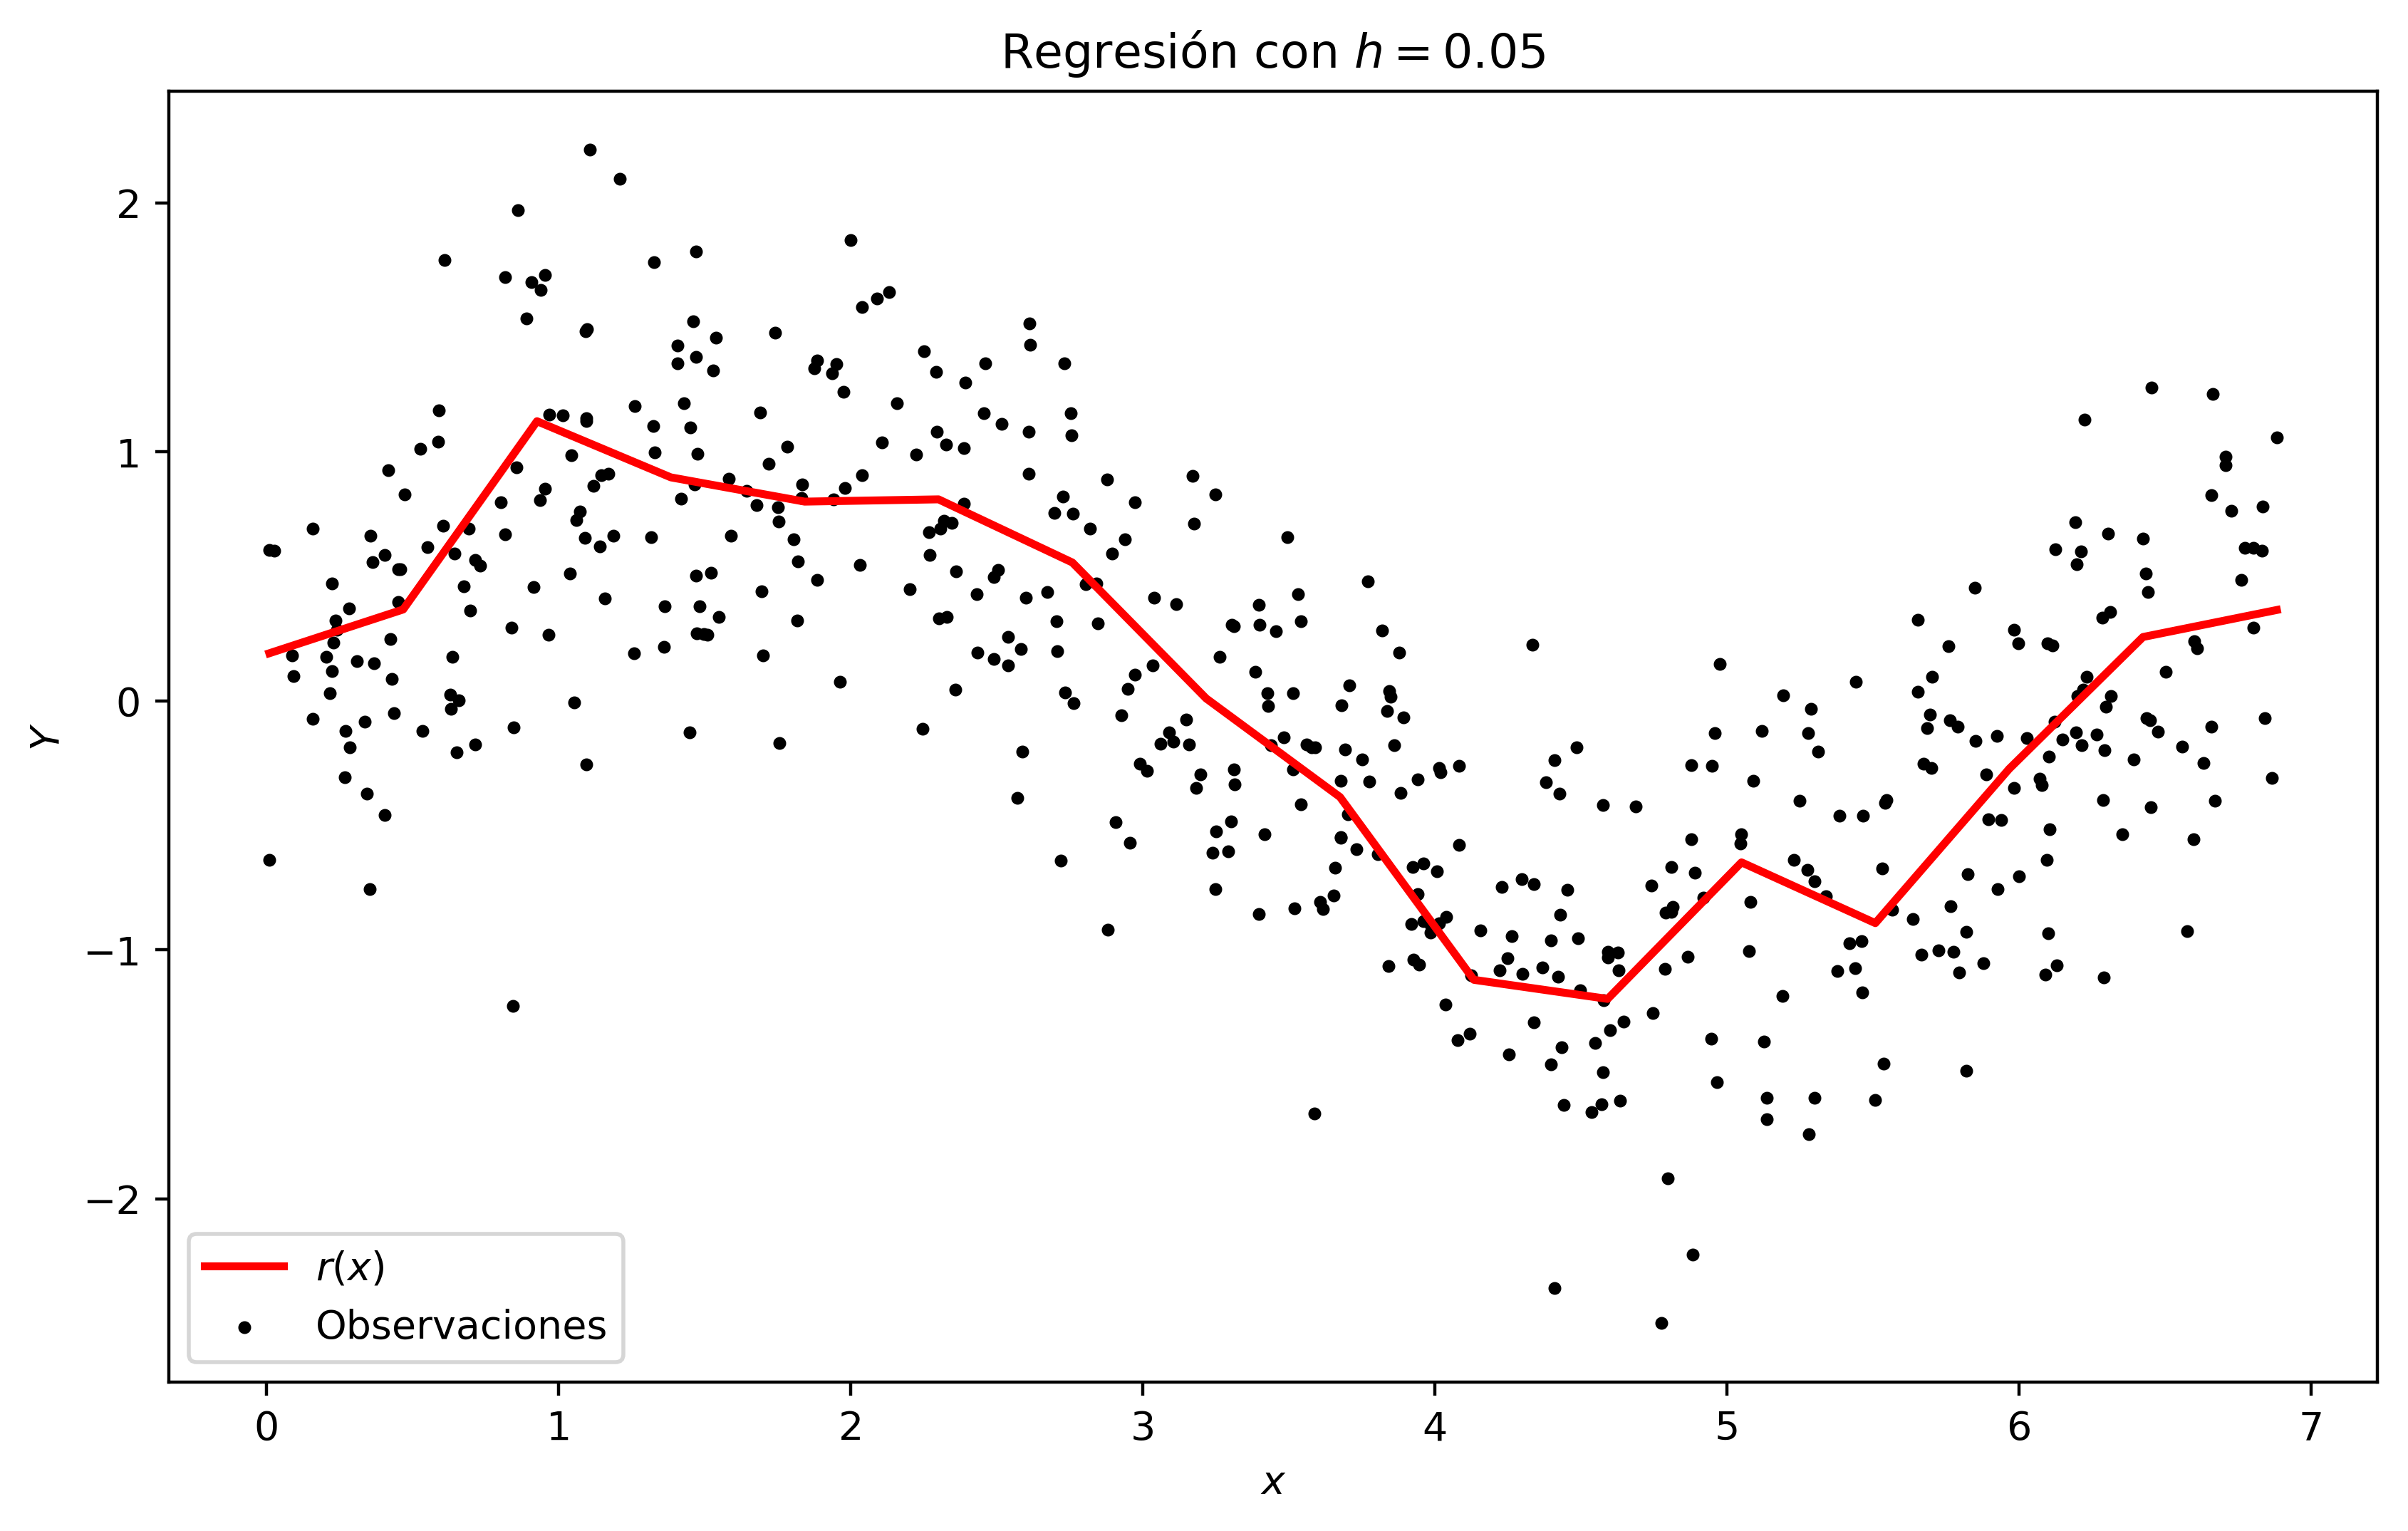
\includegraphics[scale=0.5]{regresion7}
\end{frame}

\begin{frame}
\section{Validación cruzada}
\frametitle{Validación cruzada}
Para poder seleccionar nuestro parámetro de suavizamiento necesitamos de un criterio con el que podamos medir el error que estamos cometiendo al estimar $r$, nuestro error lo podemos medir como $$R(h)=\mathbb{E}\left(\frac{1}{n}\sum_{i=1}^{n}(\hat{r}_n(x_i)-r(x_i))^2\right)$$
Debido a que $R$ depende de $r$ no podemos minimizar directamente $R$, en lugar de eso, buscaremos minimizar $$\hat{R}(h)=\frac{1}{n}\sum_{i=1}^{n}(Y_i-\hat{r}_n(x_i))^2$$
\end{frame}



\begin{frame}
\frametitle{Validación cruzada}
Sin embargo está estimación resulta no ser muy efectiva, de alguna forma sobreajusta al momento de comparar $\hat{r}_n(x_i)$ con $Y_i$ estamos usando la información original para comparar. Para medir el riesgo utilizaremos validación cruzada, excluyendo un dato a la vez:
\begin{block}{Definición}
El score de valicación cruzada esta definido como 
$$\text{cv} = \hat{R}(h) = \frac{1}{n}\sum_{i=1}^{n}(Y_i-\hat{r}_{(-i)}(x_i))^2$$
Donde $\hat{r}_{(-i)}$ es la estimación de $r$ sin utilizar la i-ésima observación $(x_i,Y_i)$
\end{block}
Con esta función de $h$ podemos buscar el valor $h$ que minimiza el error.
\end{frame}



\begin{frame}
\frametitle{Validación cruzada}
En el caso particular de los regresores linales $\hat{R}(h)$ se puede simplificar
\begin{block}{Teorema}
Si $\hat{r}_n$ es un estimador lineal entonces la validación cruzada se puede reescribir como 
$$\hat{R}(h)=\frac{1}{n}\sum_{i=1}^{n}\left(\frac{Y_i-\hat{r}_n(x_i)}{1-L_{ii}}\right)^2$$
\end{block}
\end{frame}

\begin{frame}
\section{Estimación de Kernel Nadaraya-Watson}
\frametitle{Estimación de Kernel Nadaraya-Watson}
Nos enfocaremos en el estimador de \textbf{Kernel Nadaraya-Watson}, esta estimación consiste en utilizar un Kernel $K$ y un ancho de banda $h>0$, promedio de forma ponderada cada uno de los puntos, la ponderación esta dada por la función $K$.
\begin{block}{Definición}
Sea $h>0$, se define el estimador de Kernel Nadaraya-Watson como, 
$$\hat{r}_n(x)=\sum_{i=1}^{n}\ell_i(x)Y_i$$
donde $K$ es un kernel y, 
$$\ell_i(x)=\frac{K\left(\frac{x-x_i}{h}\right)}{\sum_{j=1}^{n}K\left(\frac{x-x_j}{h}\right)} $$

\end{block}
\end{frame}



\begin{frame}
\frametitle{Estimación de Kernel Nadaraya-Watson}
\center
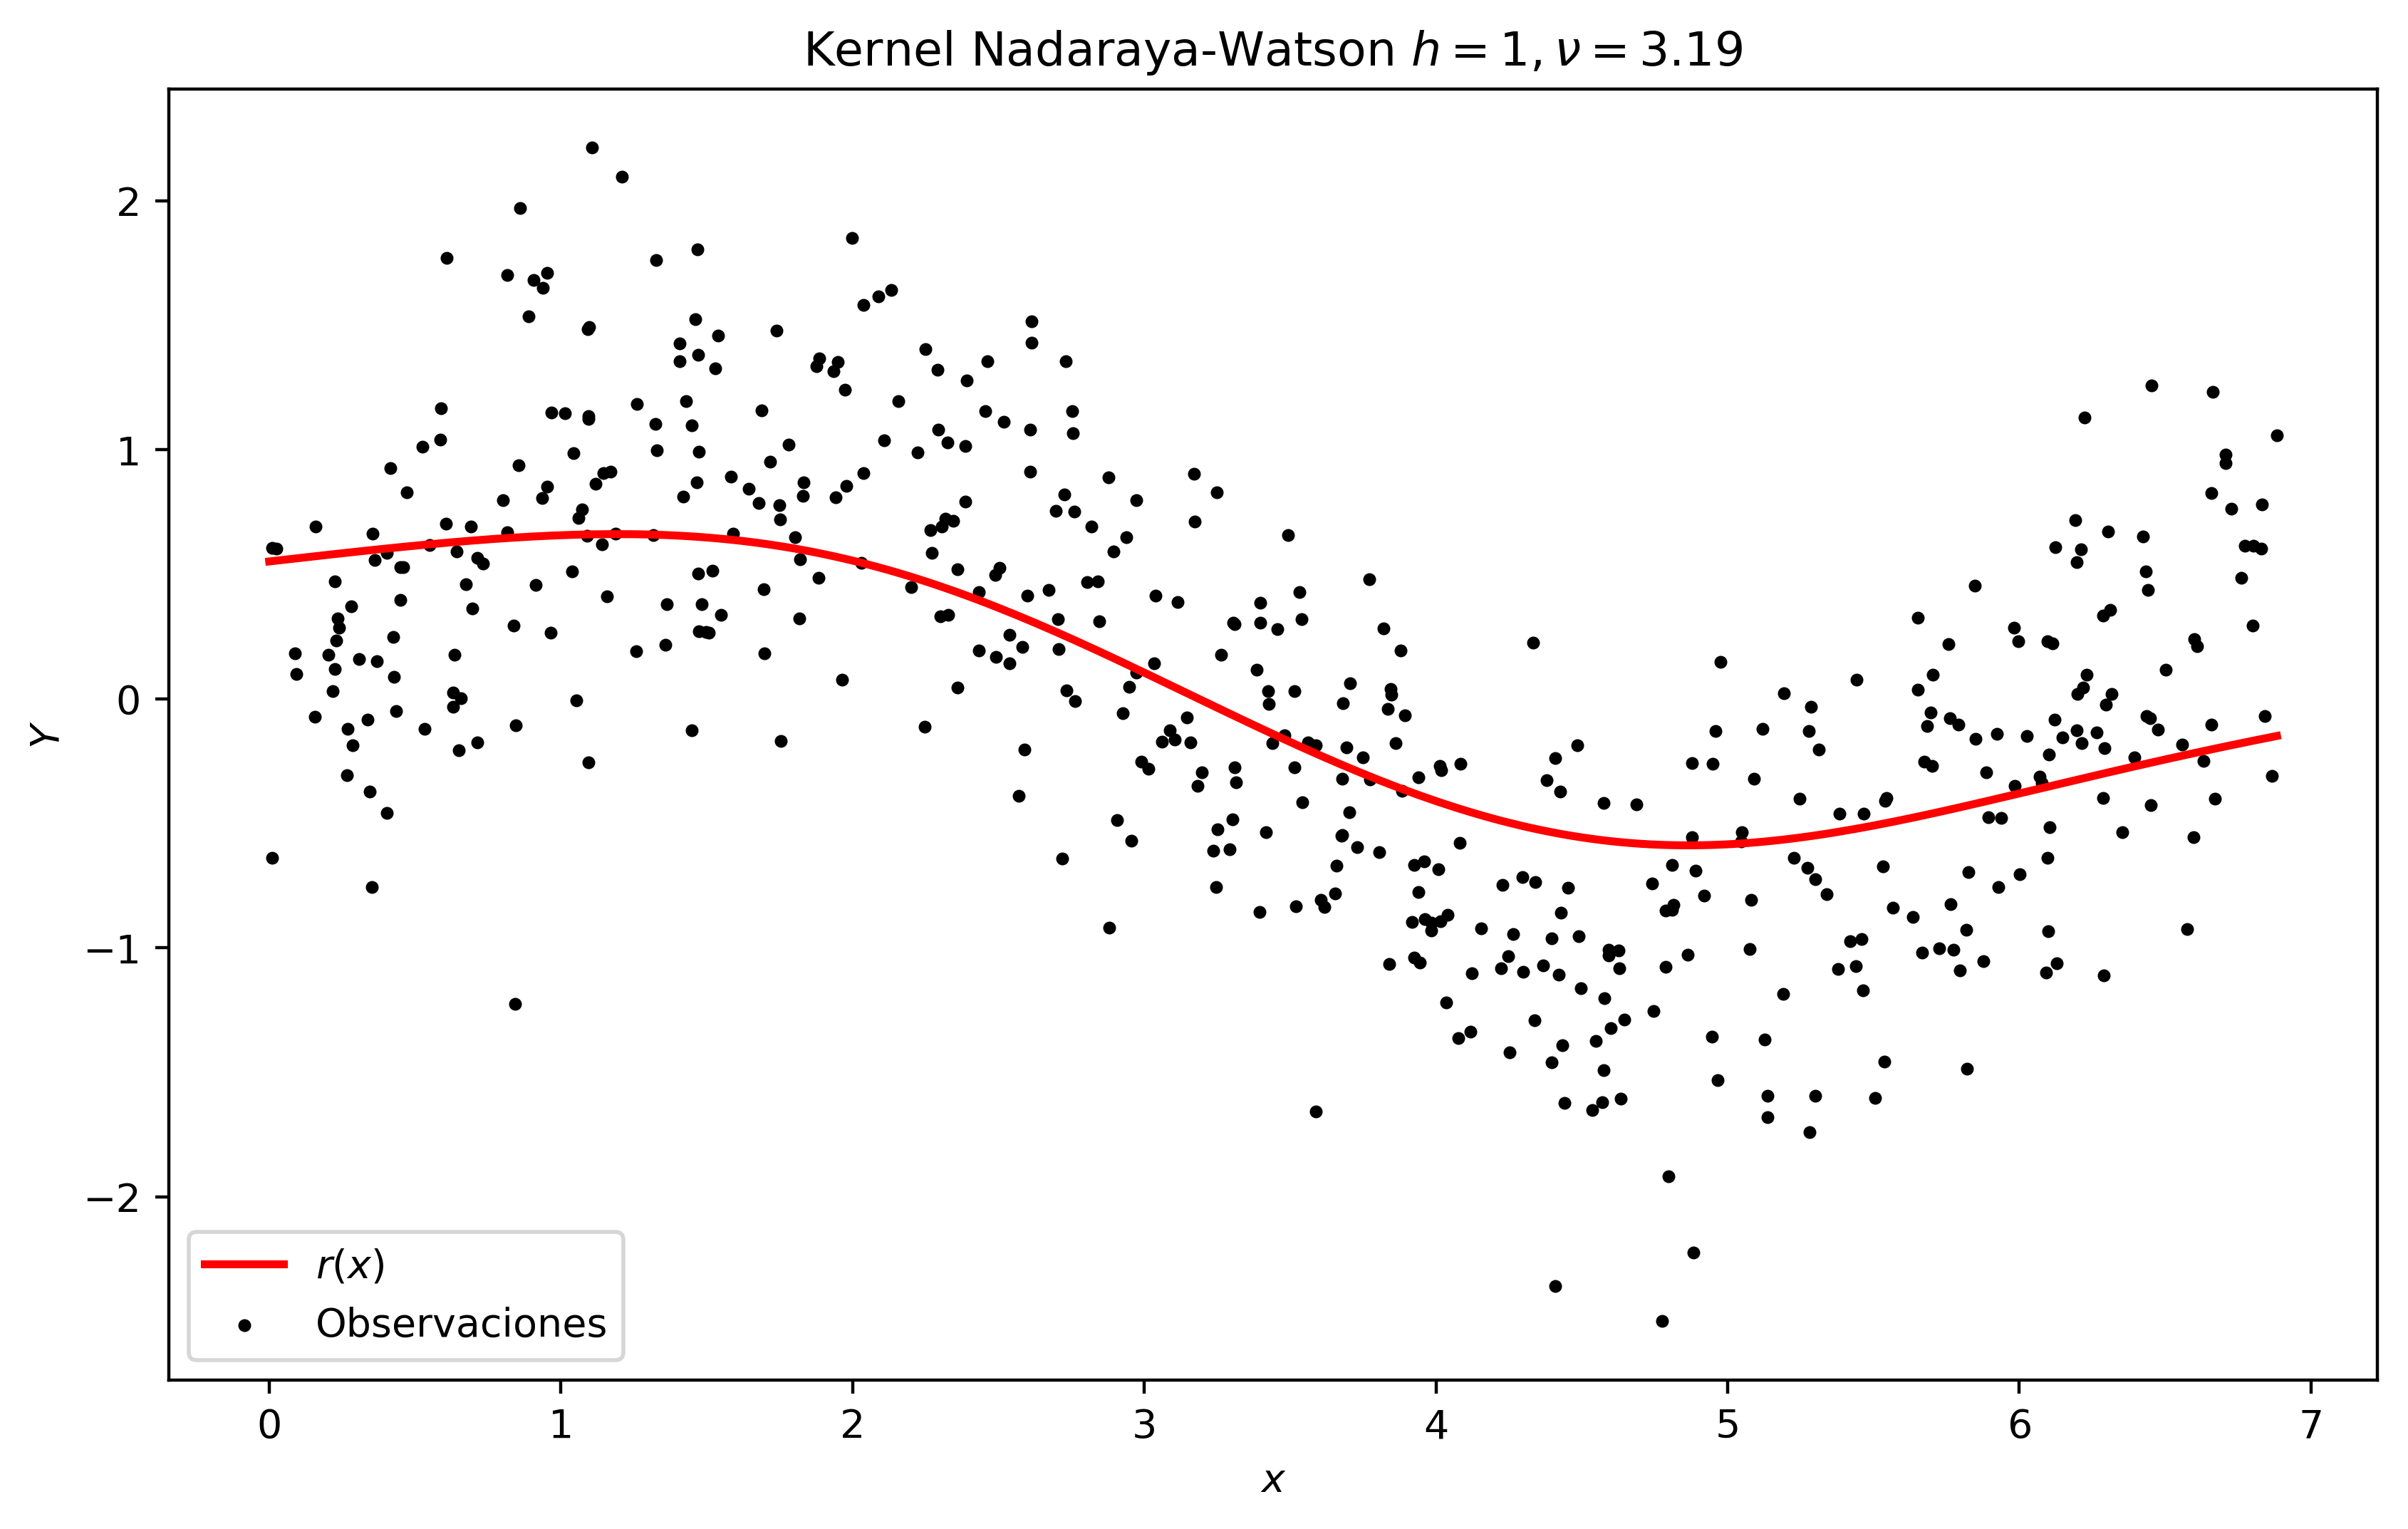
\includegraphics[scale=0.5]{regresion8}
\end{frame}


\begin{frame}
\frametitle{Estimación de Kernel Nadaraya-Watson}
\center
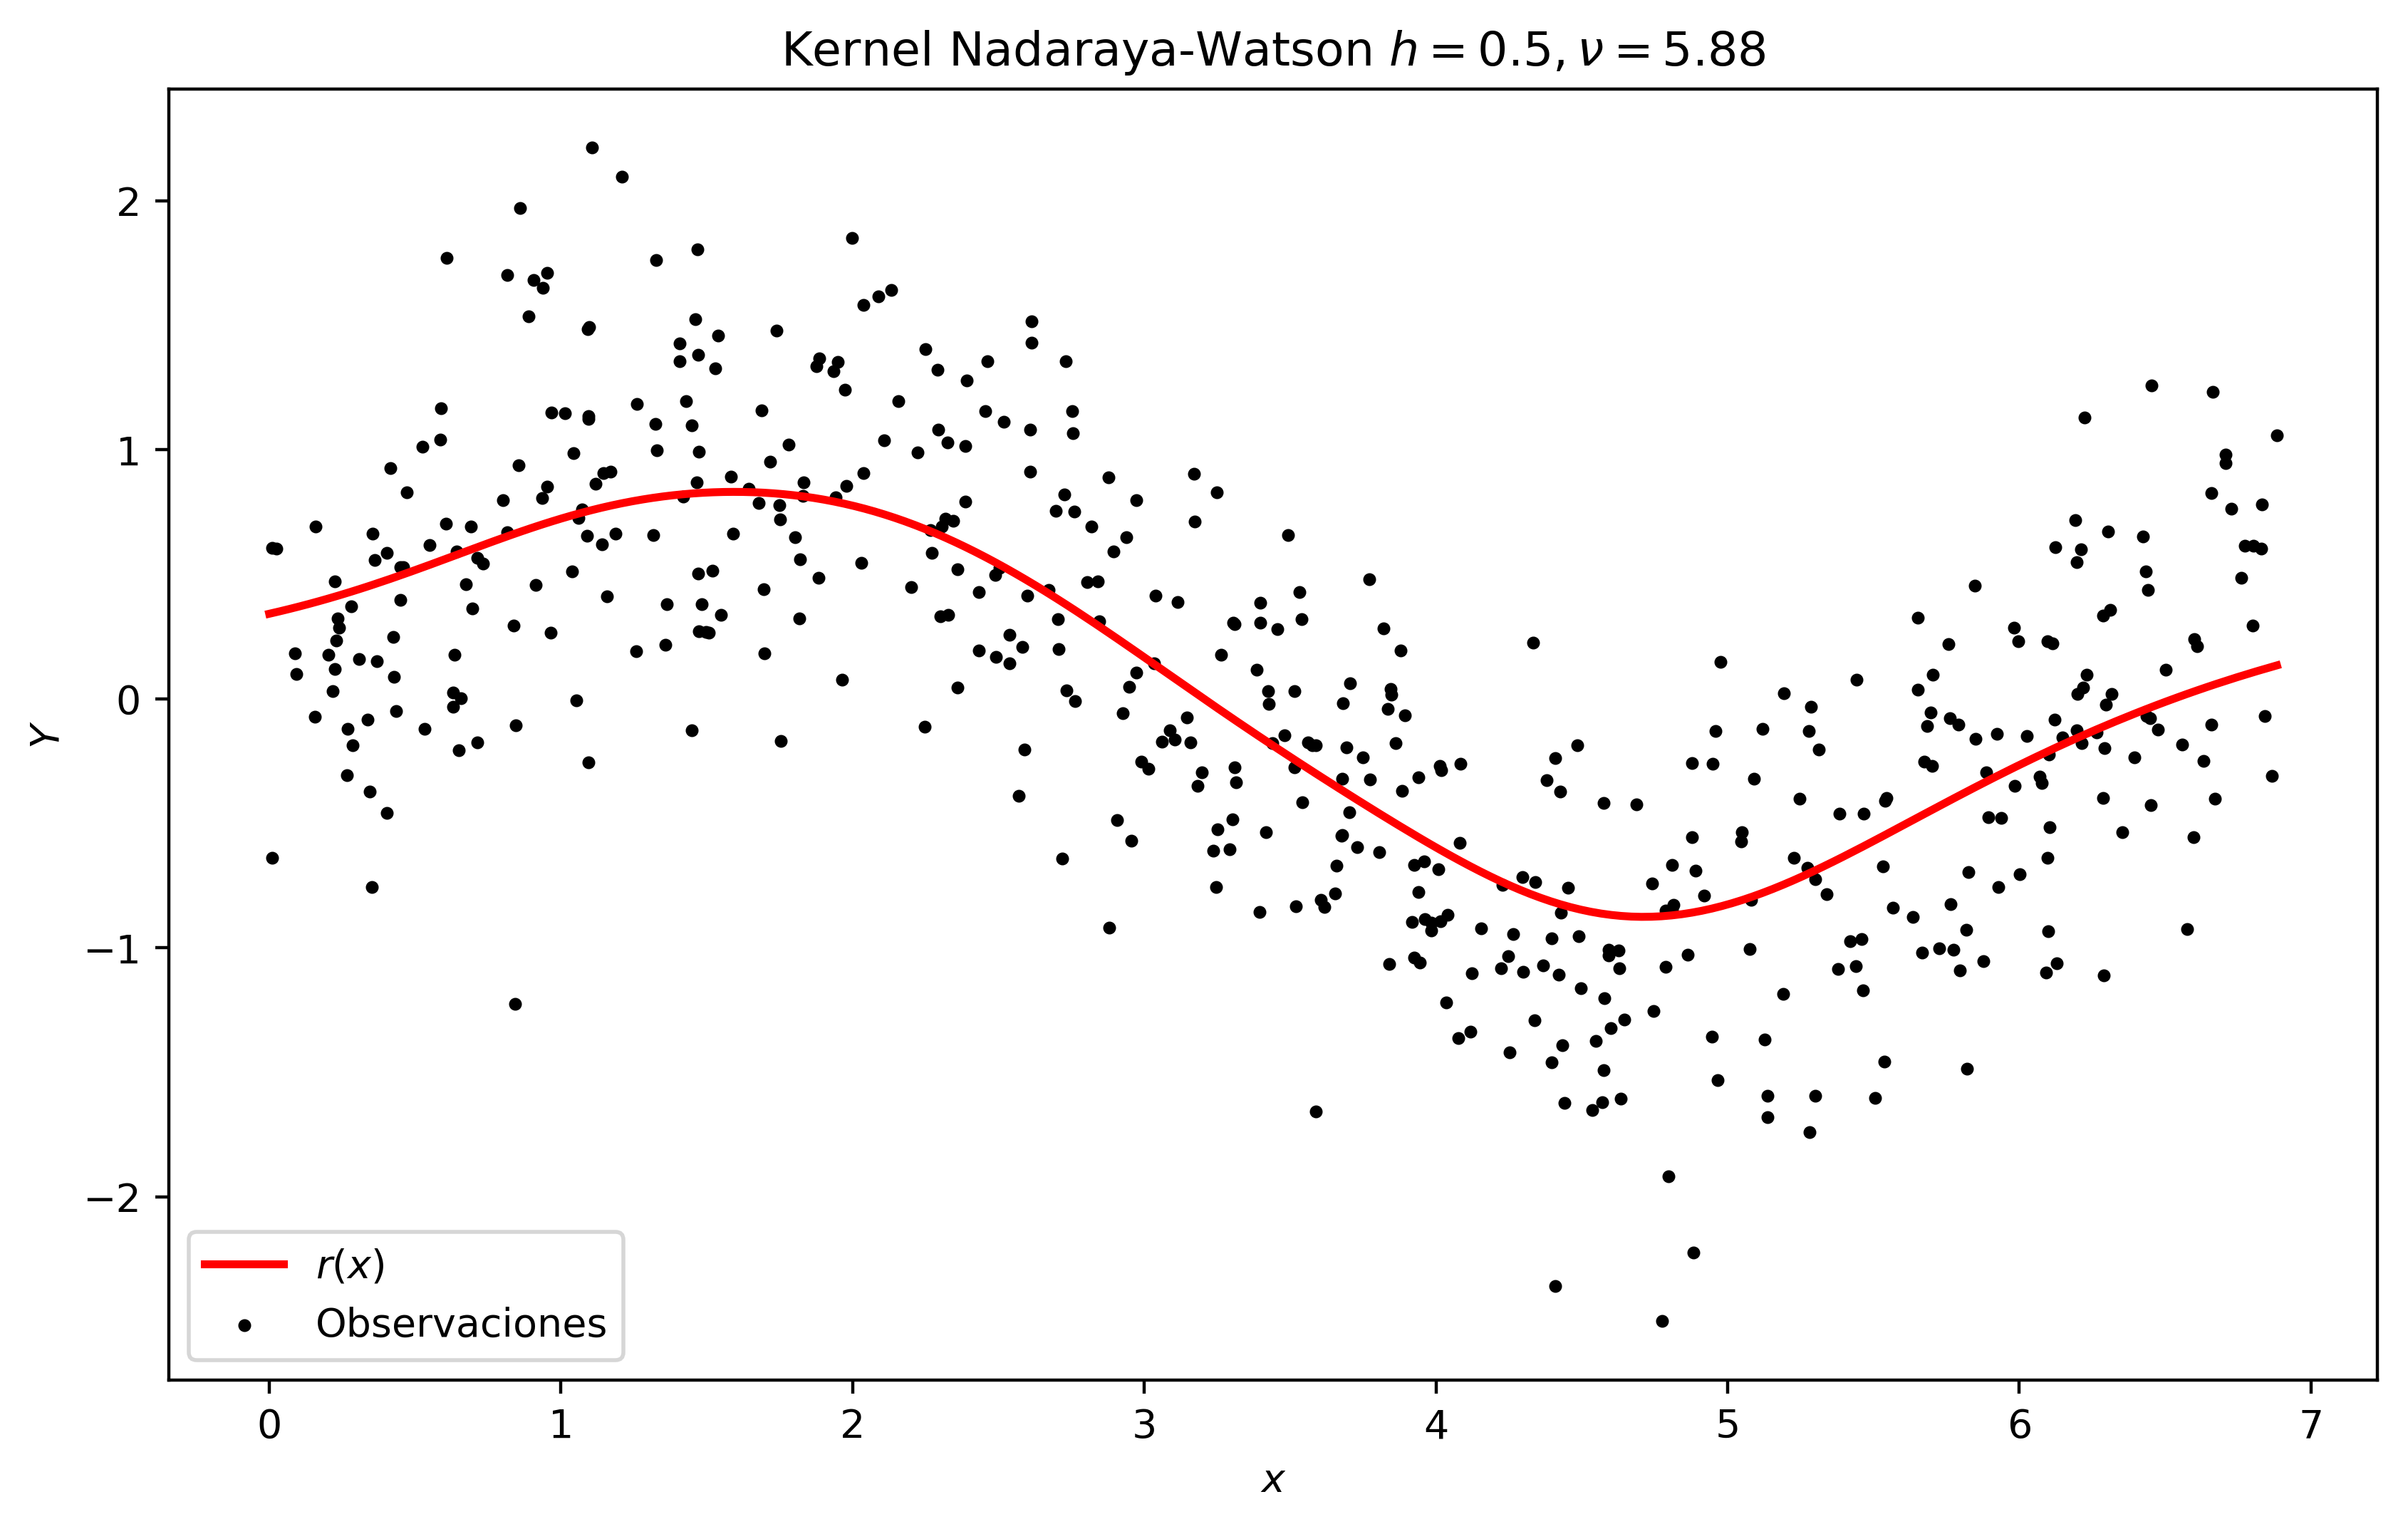
\includegraphics[scale=0.5]{regresion9}
\end{frame}


\begin{frame}
\frametitle{Estimación de Kernel Nadaraya-Watson}
\center
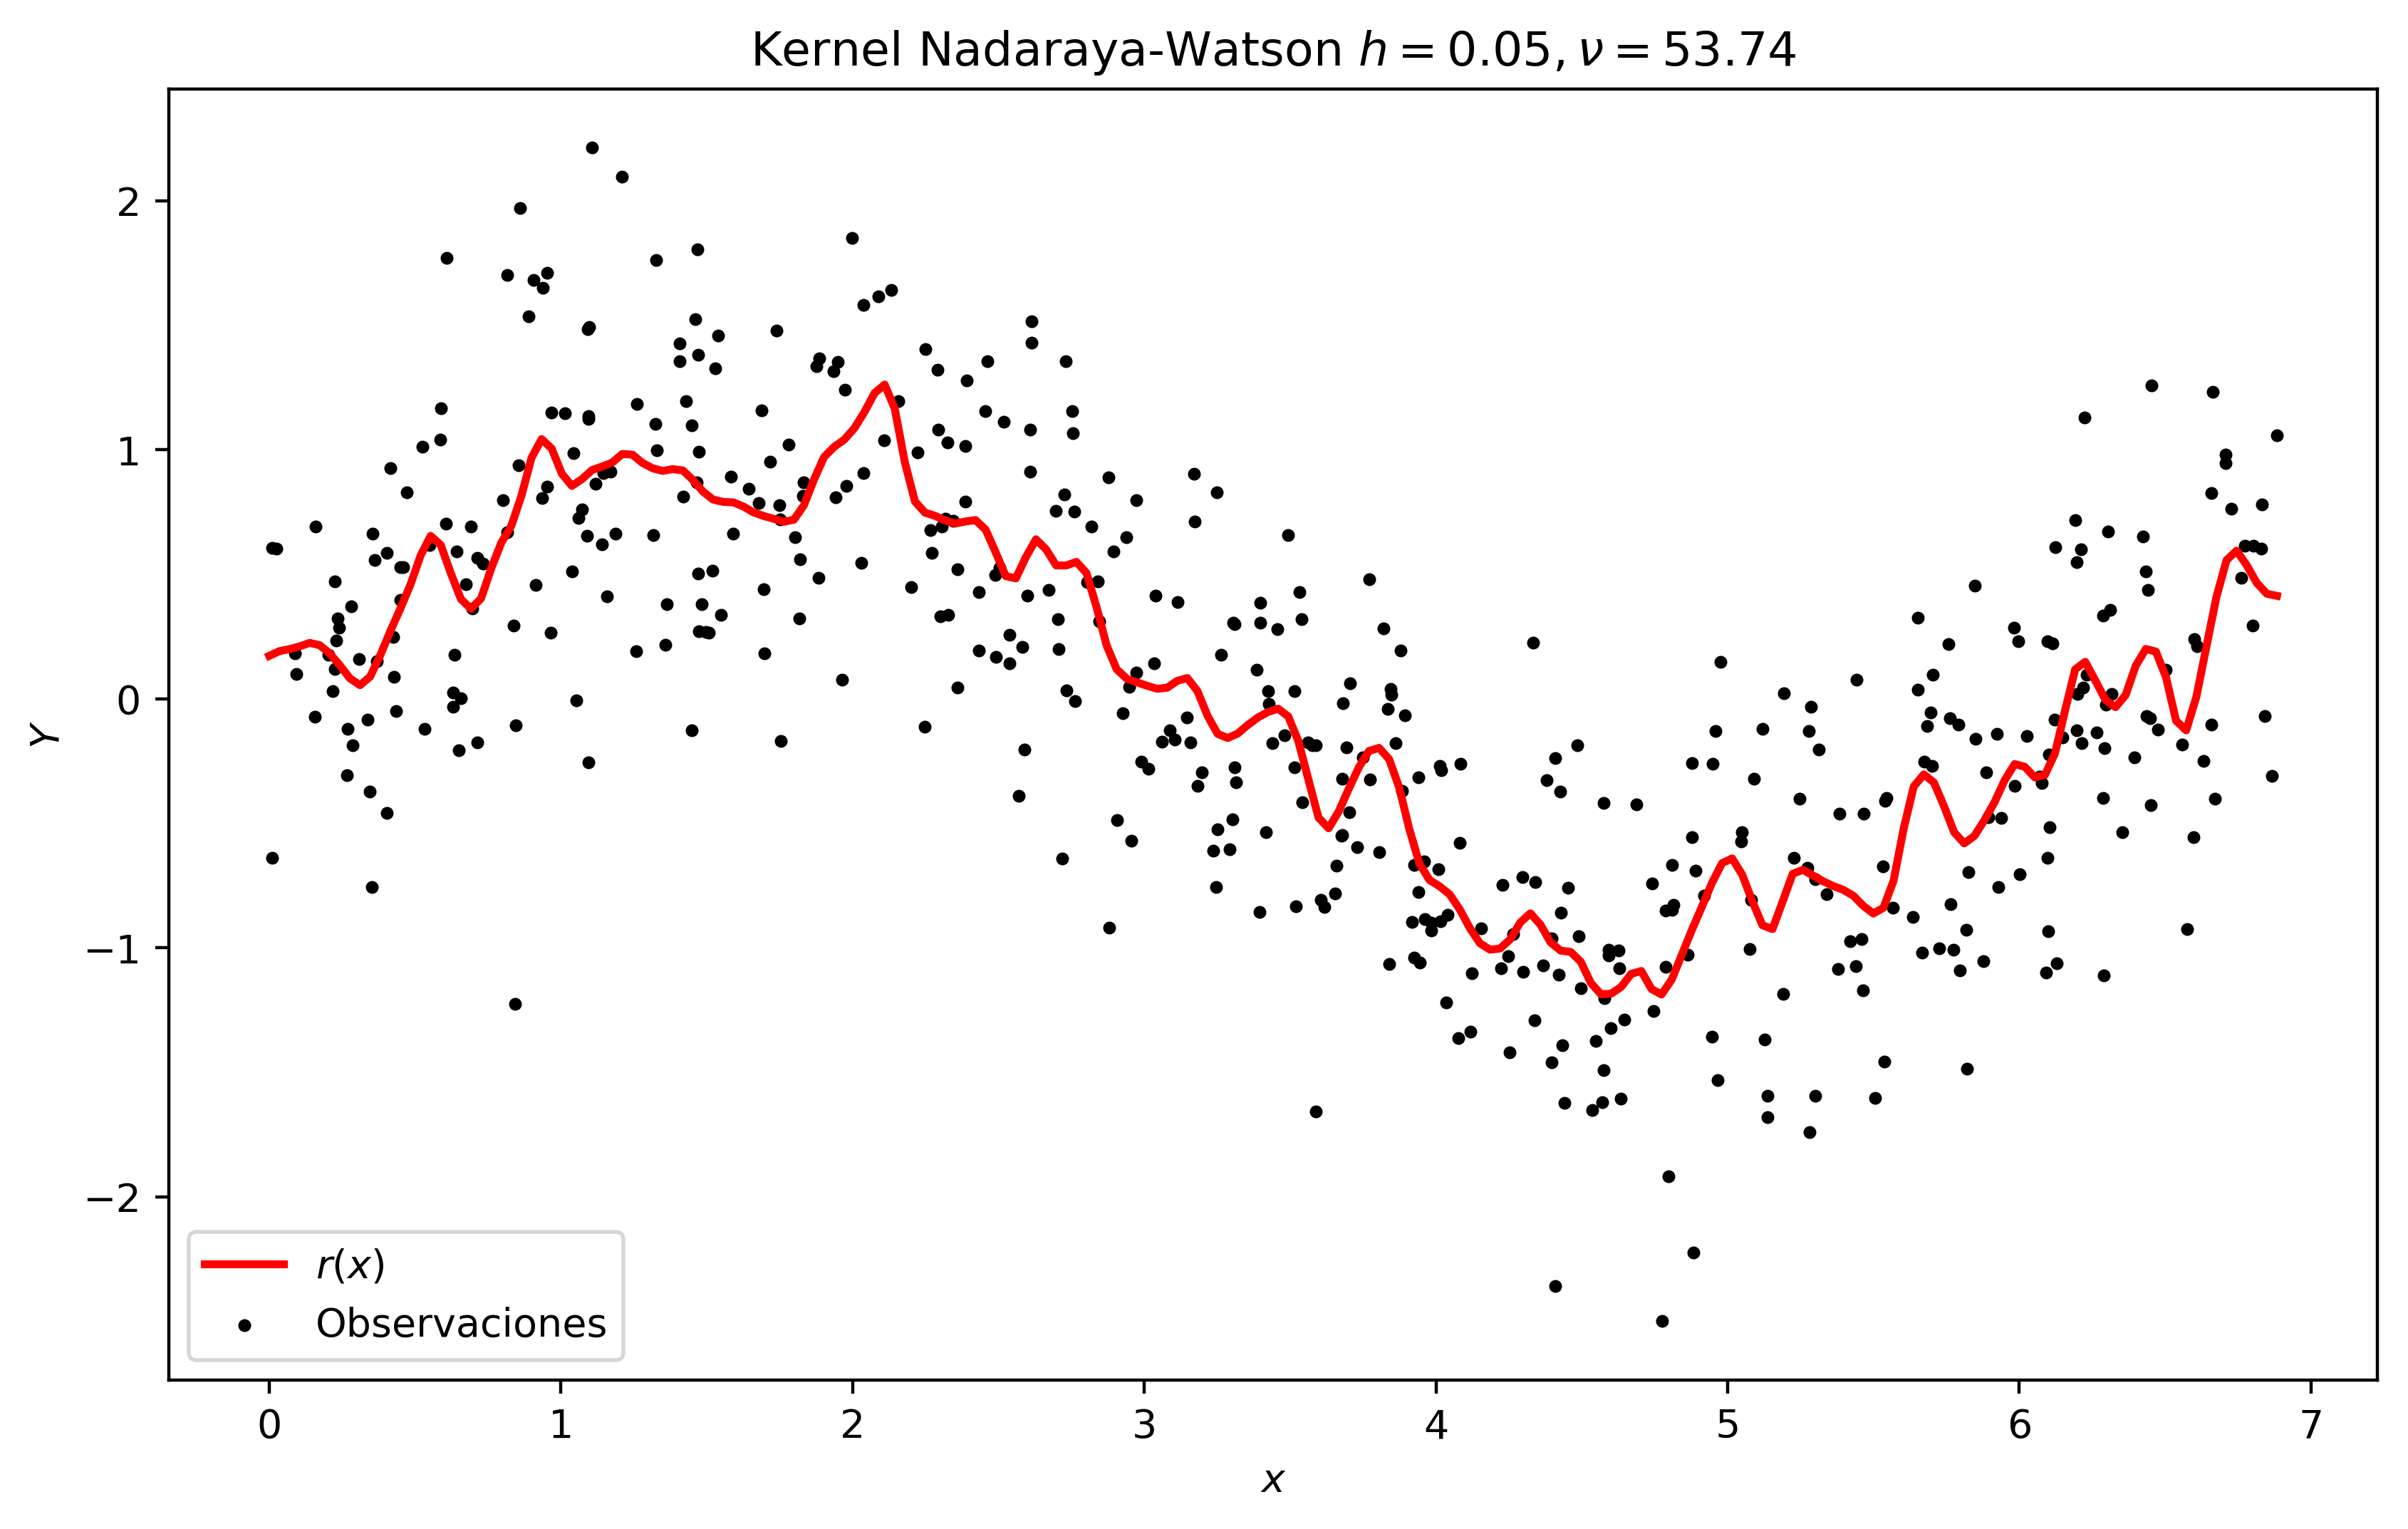
\includegraphics[scale=0.5]{regresion10}
\end{frame}

\begin{frame}
\frametitle{Estimación de Kernel Nadaraya-Watson}
\center
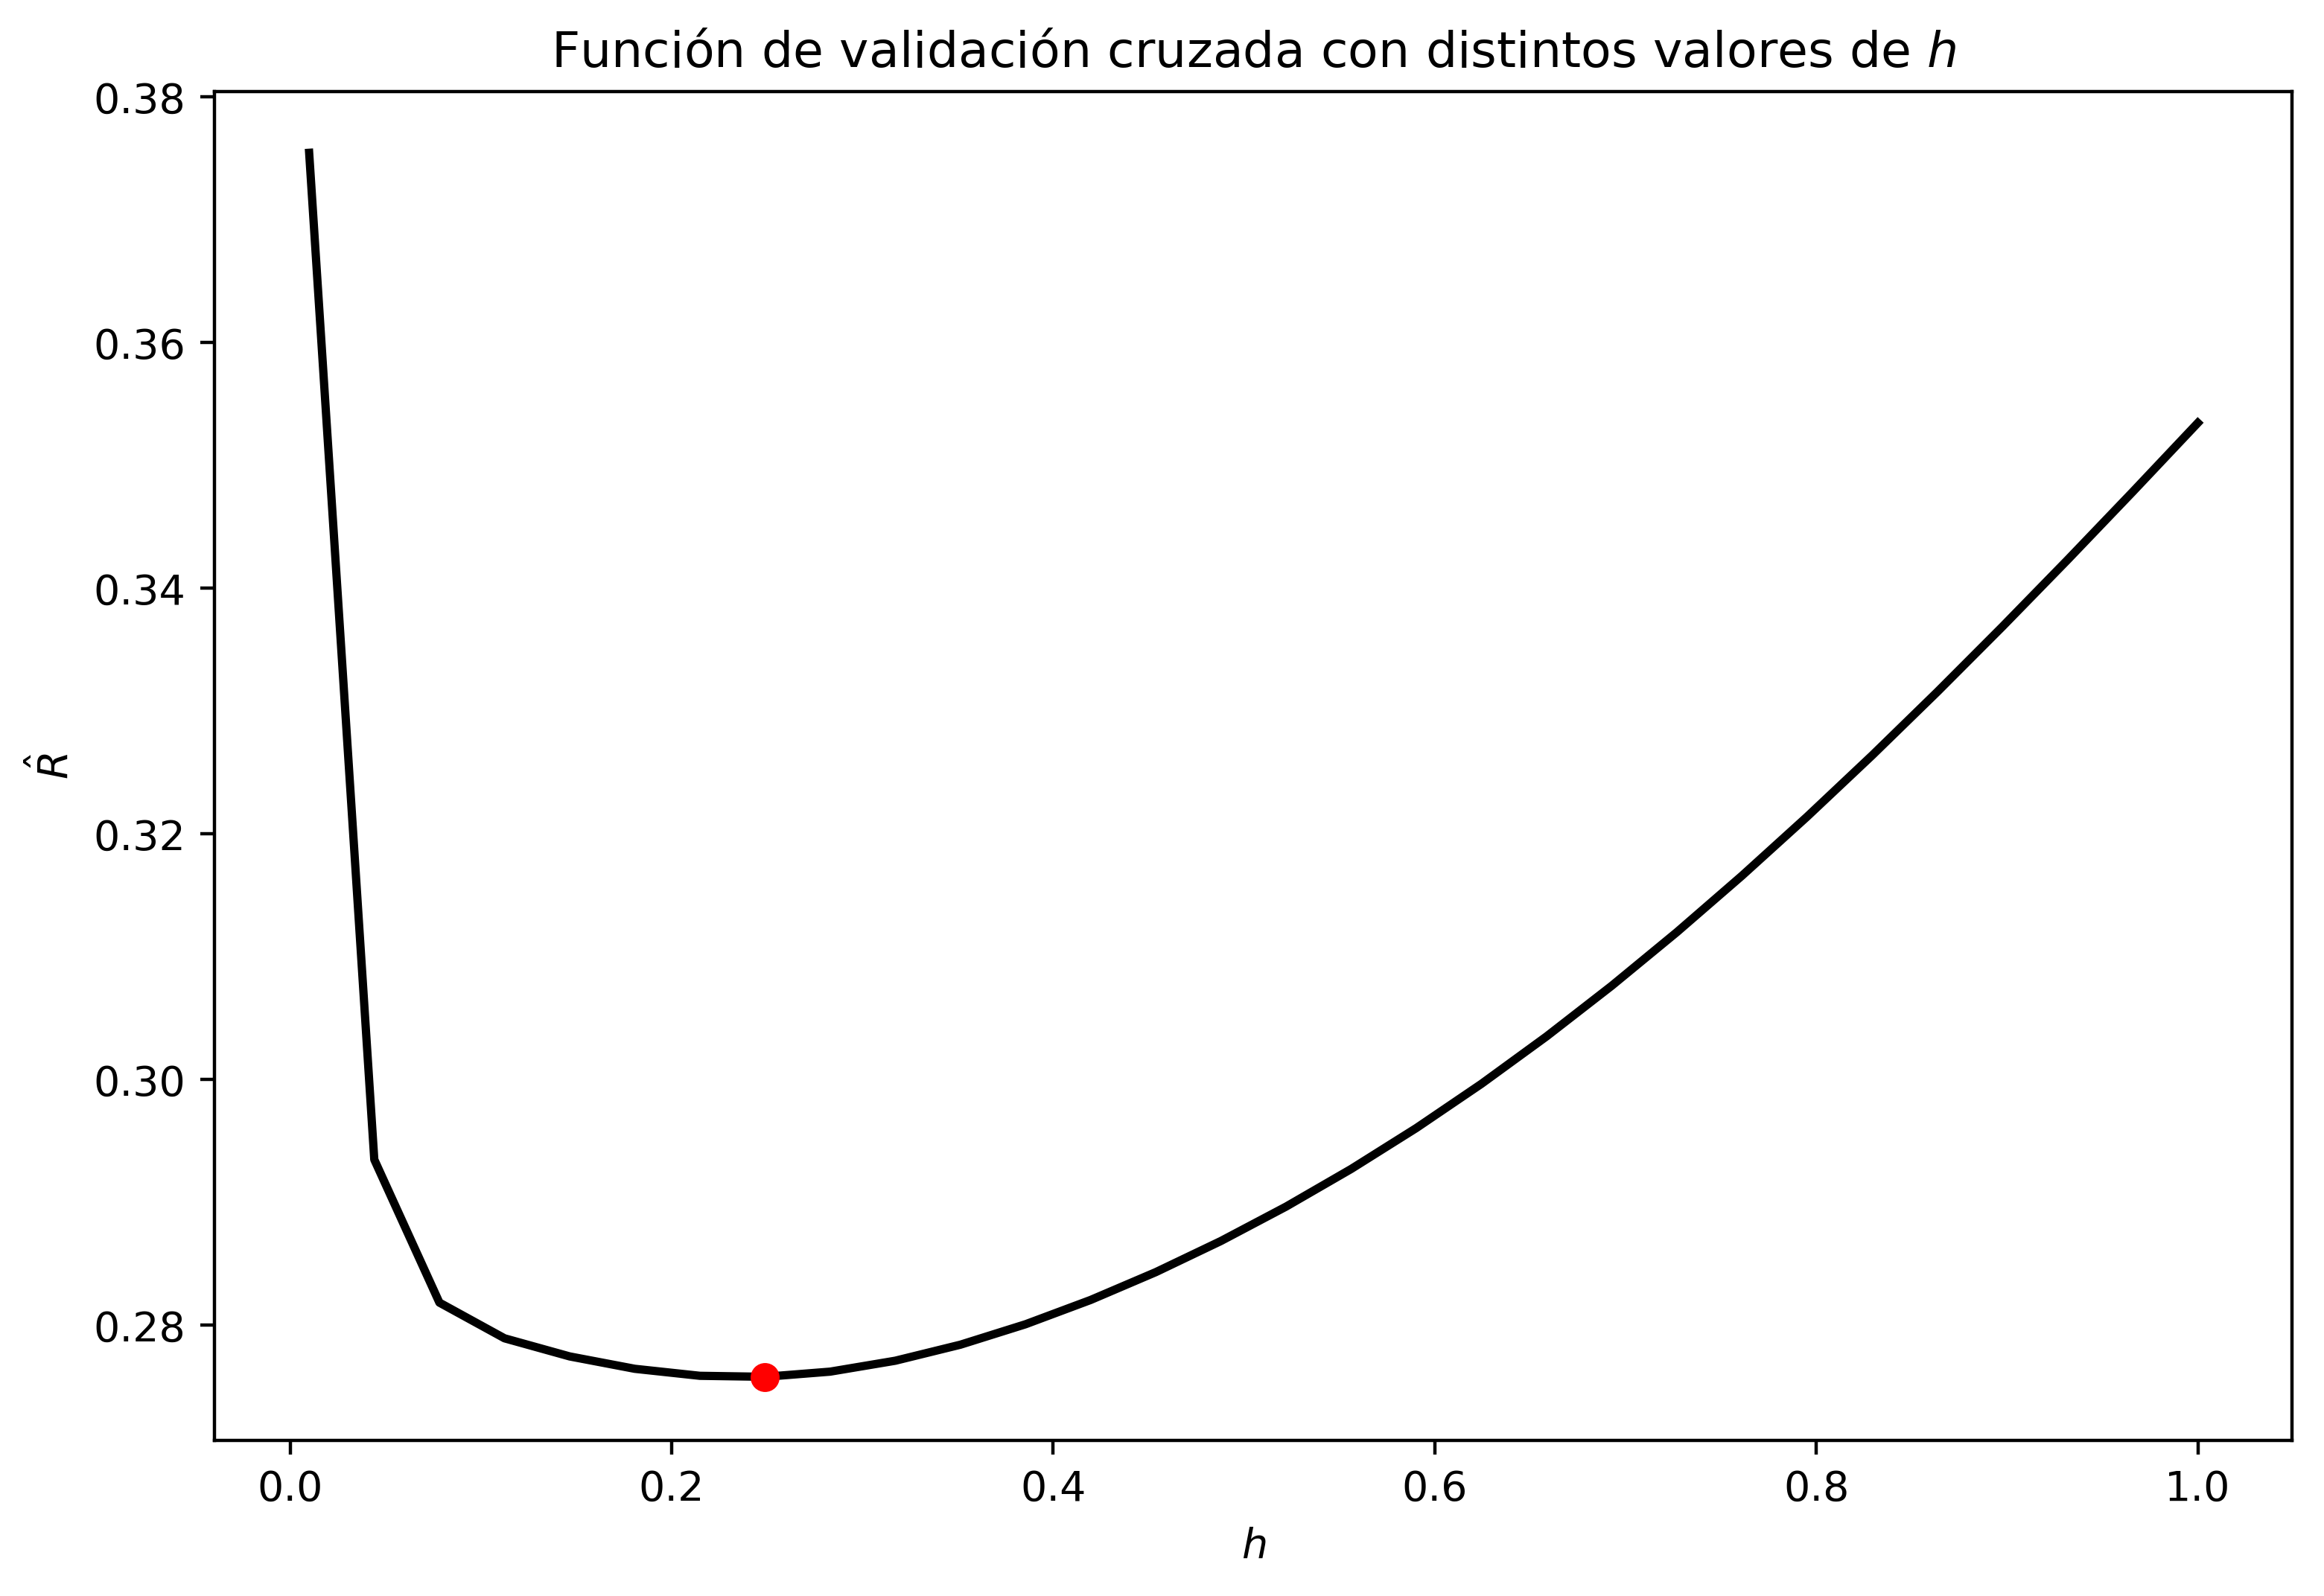
\includegraphics[scale=0.5]{cv1}
\end{frame}

\begin{frame}
\frametitle{Estimación de Kernel Nadaraya-Watson}
\center
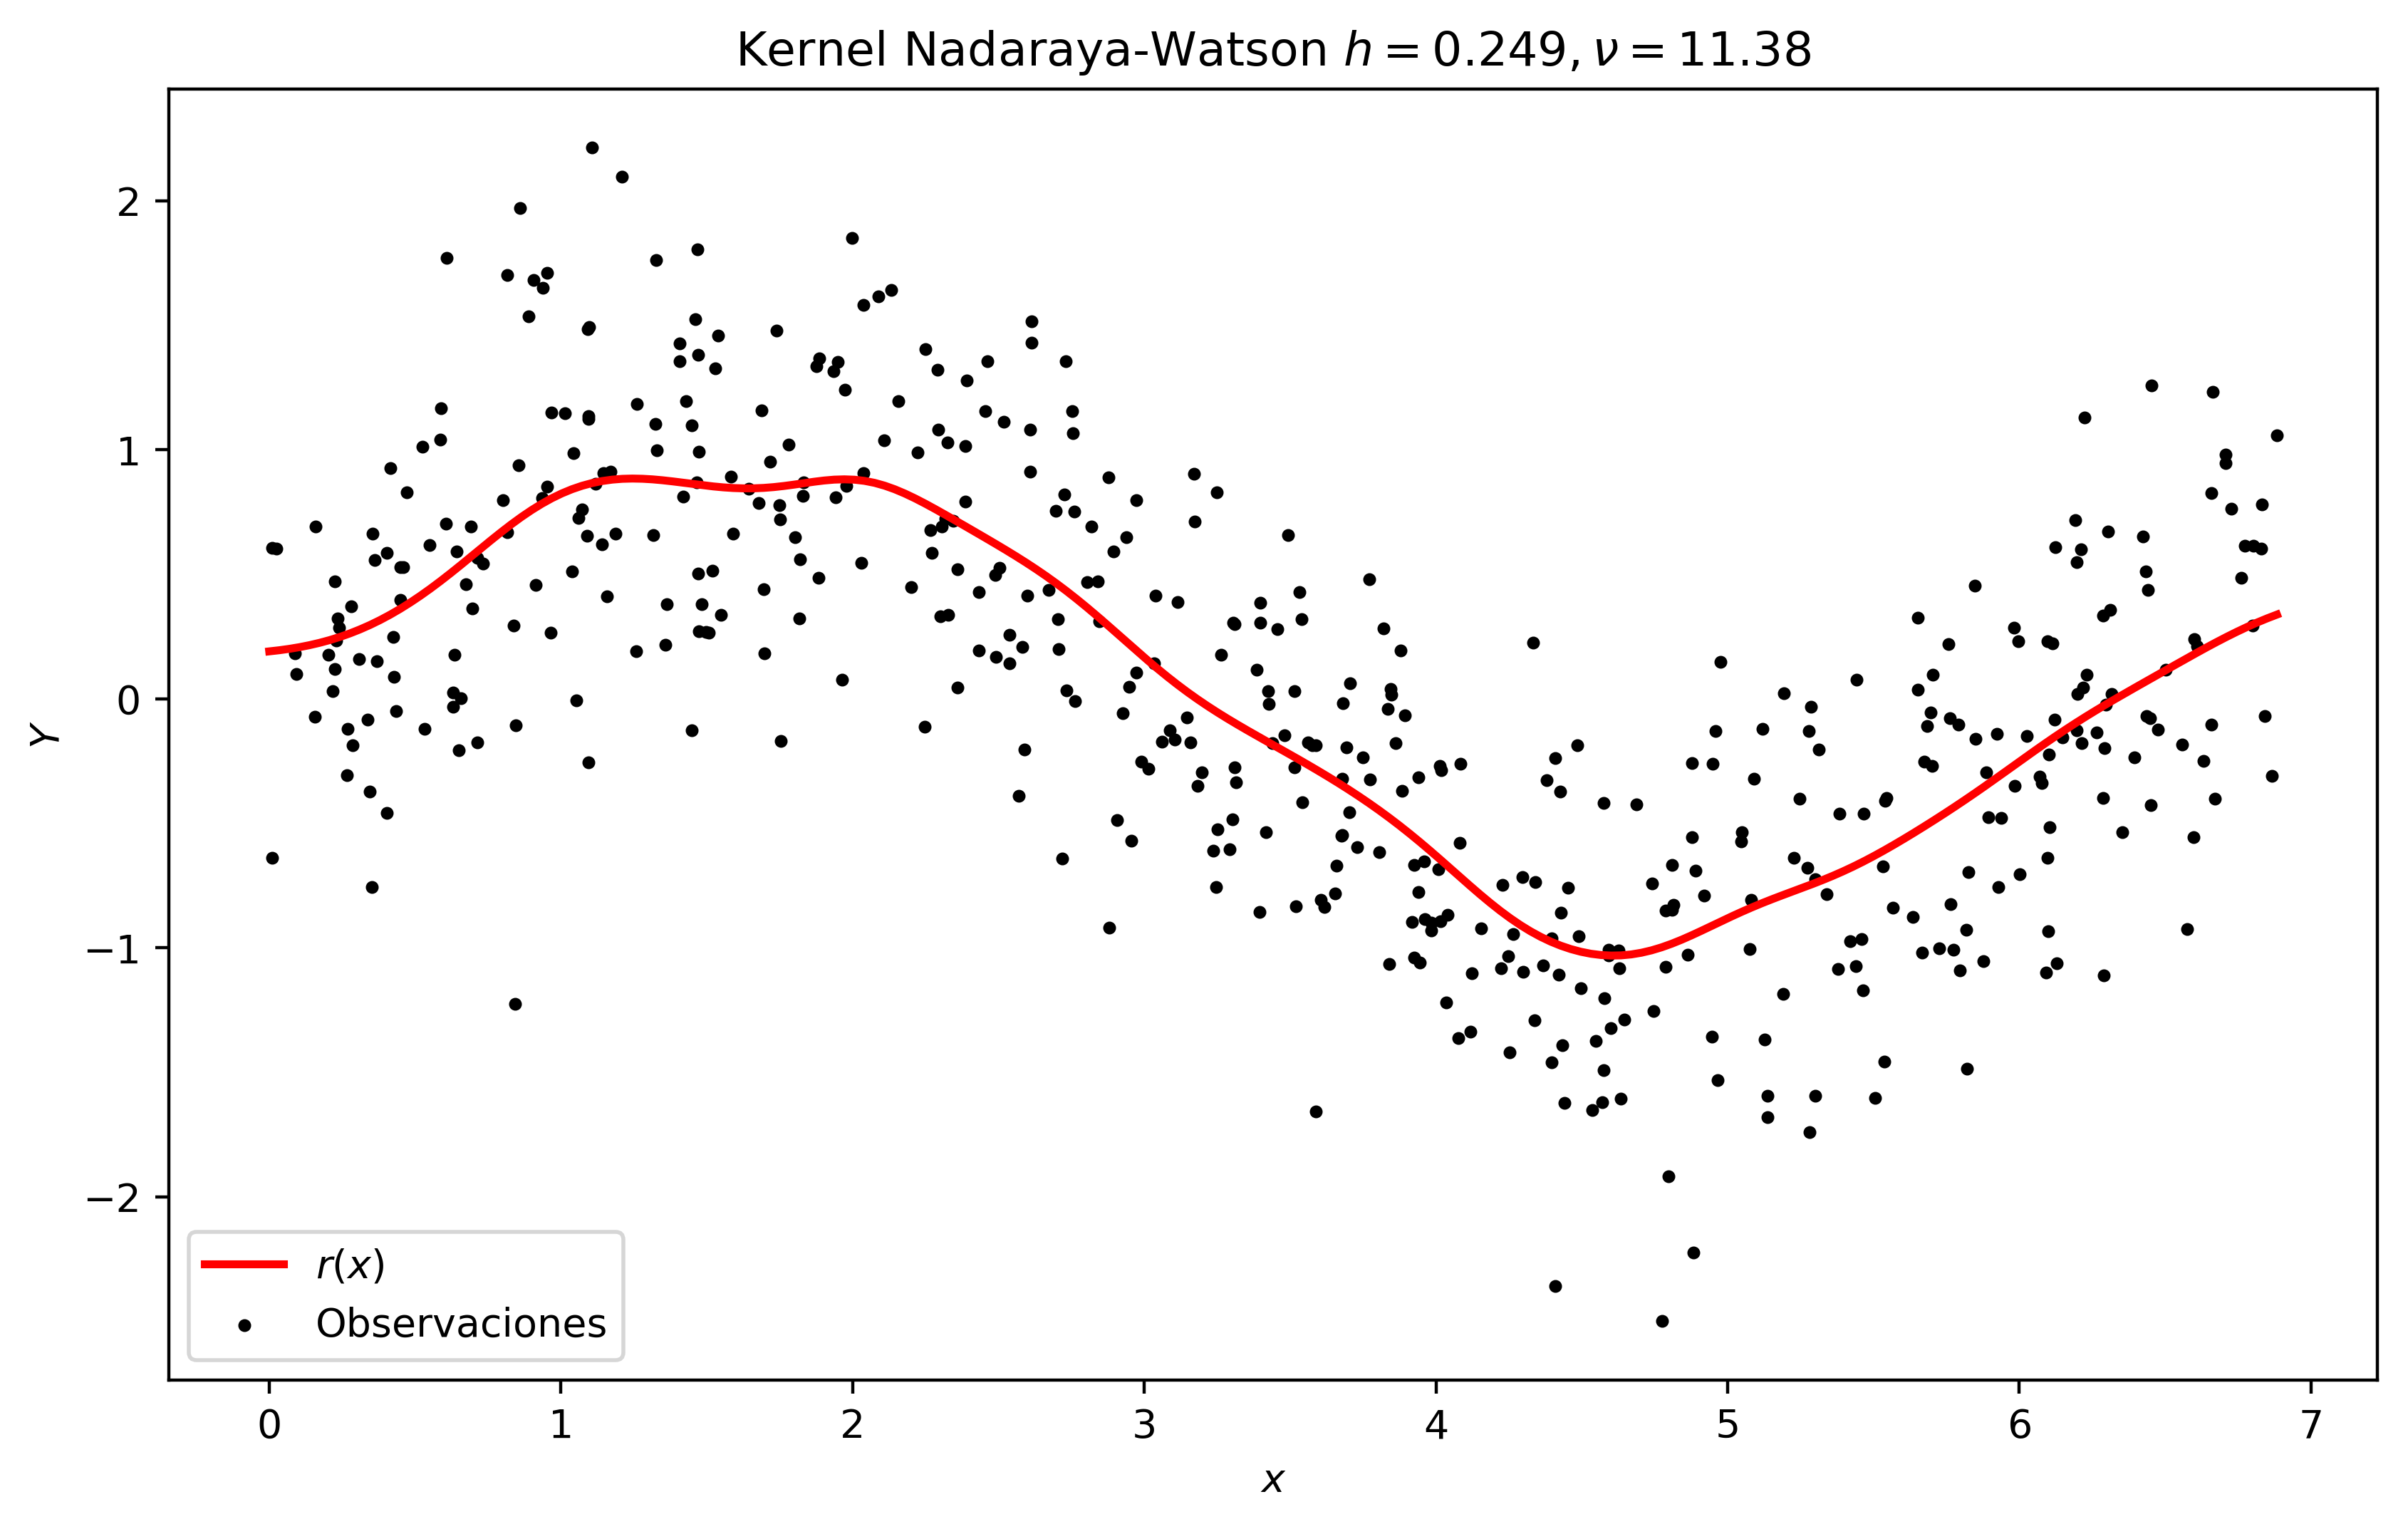
\includegraphics[scale=0.5]{regresionOp}
\end{frame}

\begin{frame}
\section{Estimación de $\sigma^{2}(x)$}
\frametitle{Estimación de $\sigma^{2}(x)$}
En el ejemplo que hemos considerado la varianza tiene un comportamiento homocedastico, si suponemos que la varianza de nuestro modelo es constante, es decir $\sigma^2=\text{Var}(\varepsilon_i)$. En esta situación podemos utilizar el siguiente estimador para regresores lineales. 
\begin{block}{Teorema}
Sea $\hat{r}_n$ un regresor lineal y sea $$\hat{\sigma^2}=\frac{\sum_{i=1}^{n}(Y_i-\hat{r}_n(x_i))^2}{n-2\nu+\tilde{\nu}}$$
Donde $\nu = \text{tr}(L)$ y $\tilde{\nu} = \text{tr}(L^T L)$
Si $\nu = o(n)$ y $\tilde{\nu} =o(n)$ entonces $\hat{\sigma^2}$ es un estimador consistente de $\sigma^2$
\end{block}
\end{frame}



\begin{frame}
\frametitle{Estimación de $\sigma^{2}(x)$}
En el ejemplo que hemos considerado la varianza tiene un comportamiento homocedastico, si suponemos que la varianza de nuestro modelo es constante, es decir $\sigma^2=\text{Var}(\varepsilon_i)$. En esta situación podemos utilizar el siguiente estimador para regresores lineales. 
\begin{block}{Teorema}
Sea $\hat{r}_n$ un regresor lineal y sea $$\hat{\sigma^2}=\frac{\sum_{i=1}^{n}(Y_i-\hat{r}_n(x_i))^2}{n-2\nu+\tilde{\nu}}$$
Donde $\nu = \text{tr}(L)$ y $\tilde{\nu} = \text{tr}(L^T L)$
Si $\nu = o(n)$ y $\tilde{\nu} =o(n)$ entonces $\hat{\sigma^2}$ es un estimador consistente de $\sigma^2$
\end{block}
\end{frame}

\begin{frame}
\frametitle{Estimación de $\sigma^{2}(x)$}
Sin embargo no siempre podemos asumir homocedasticidad...
\center
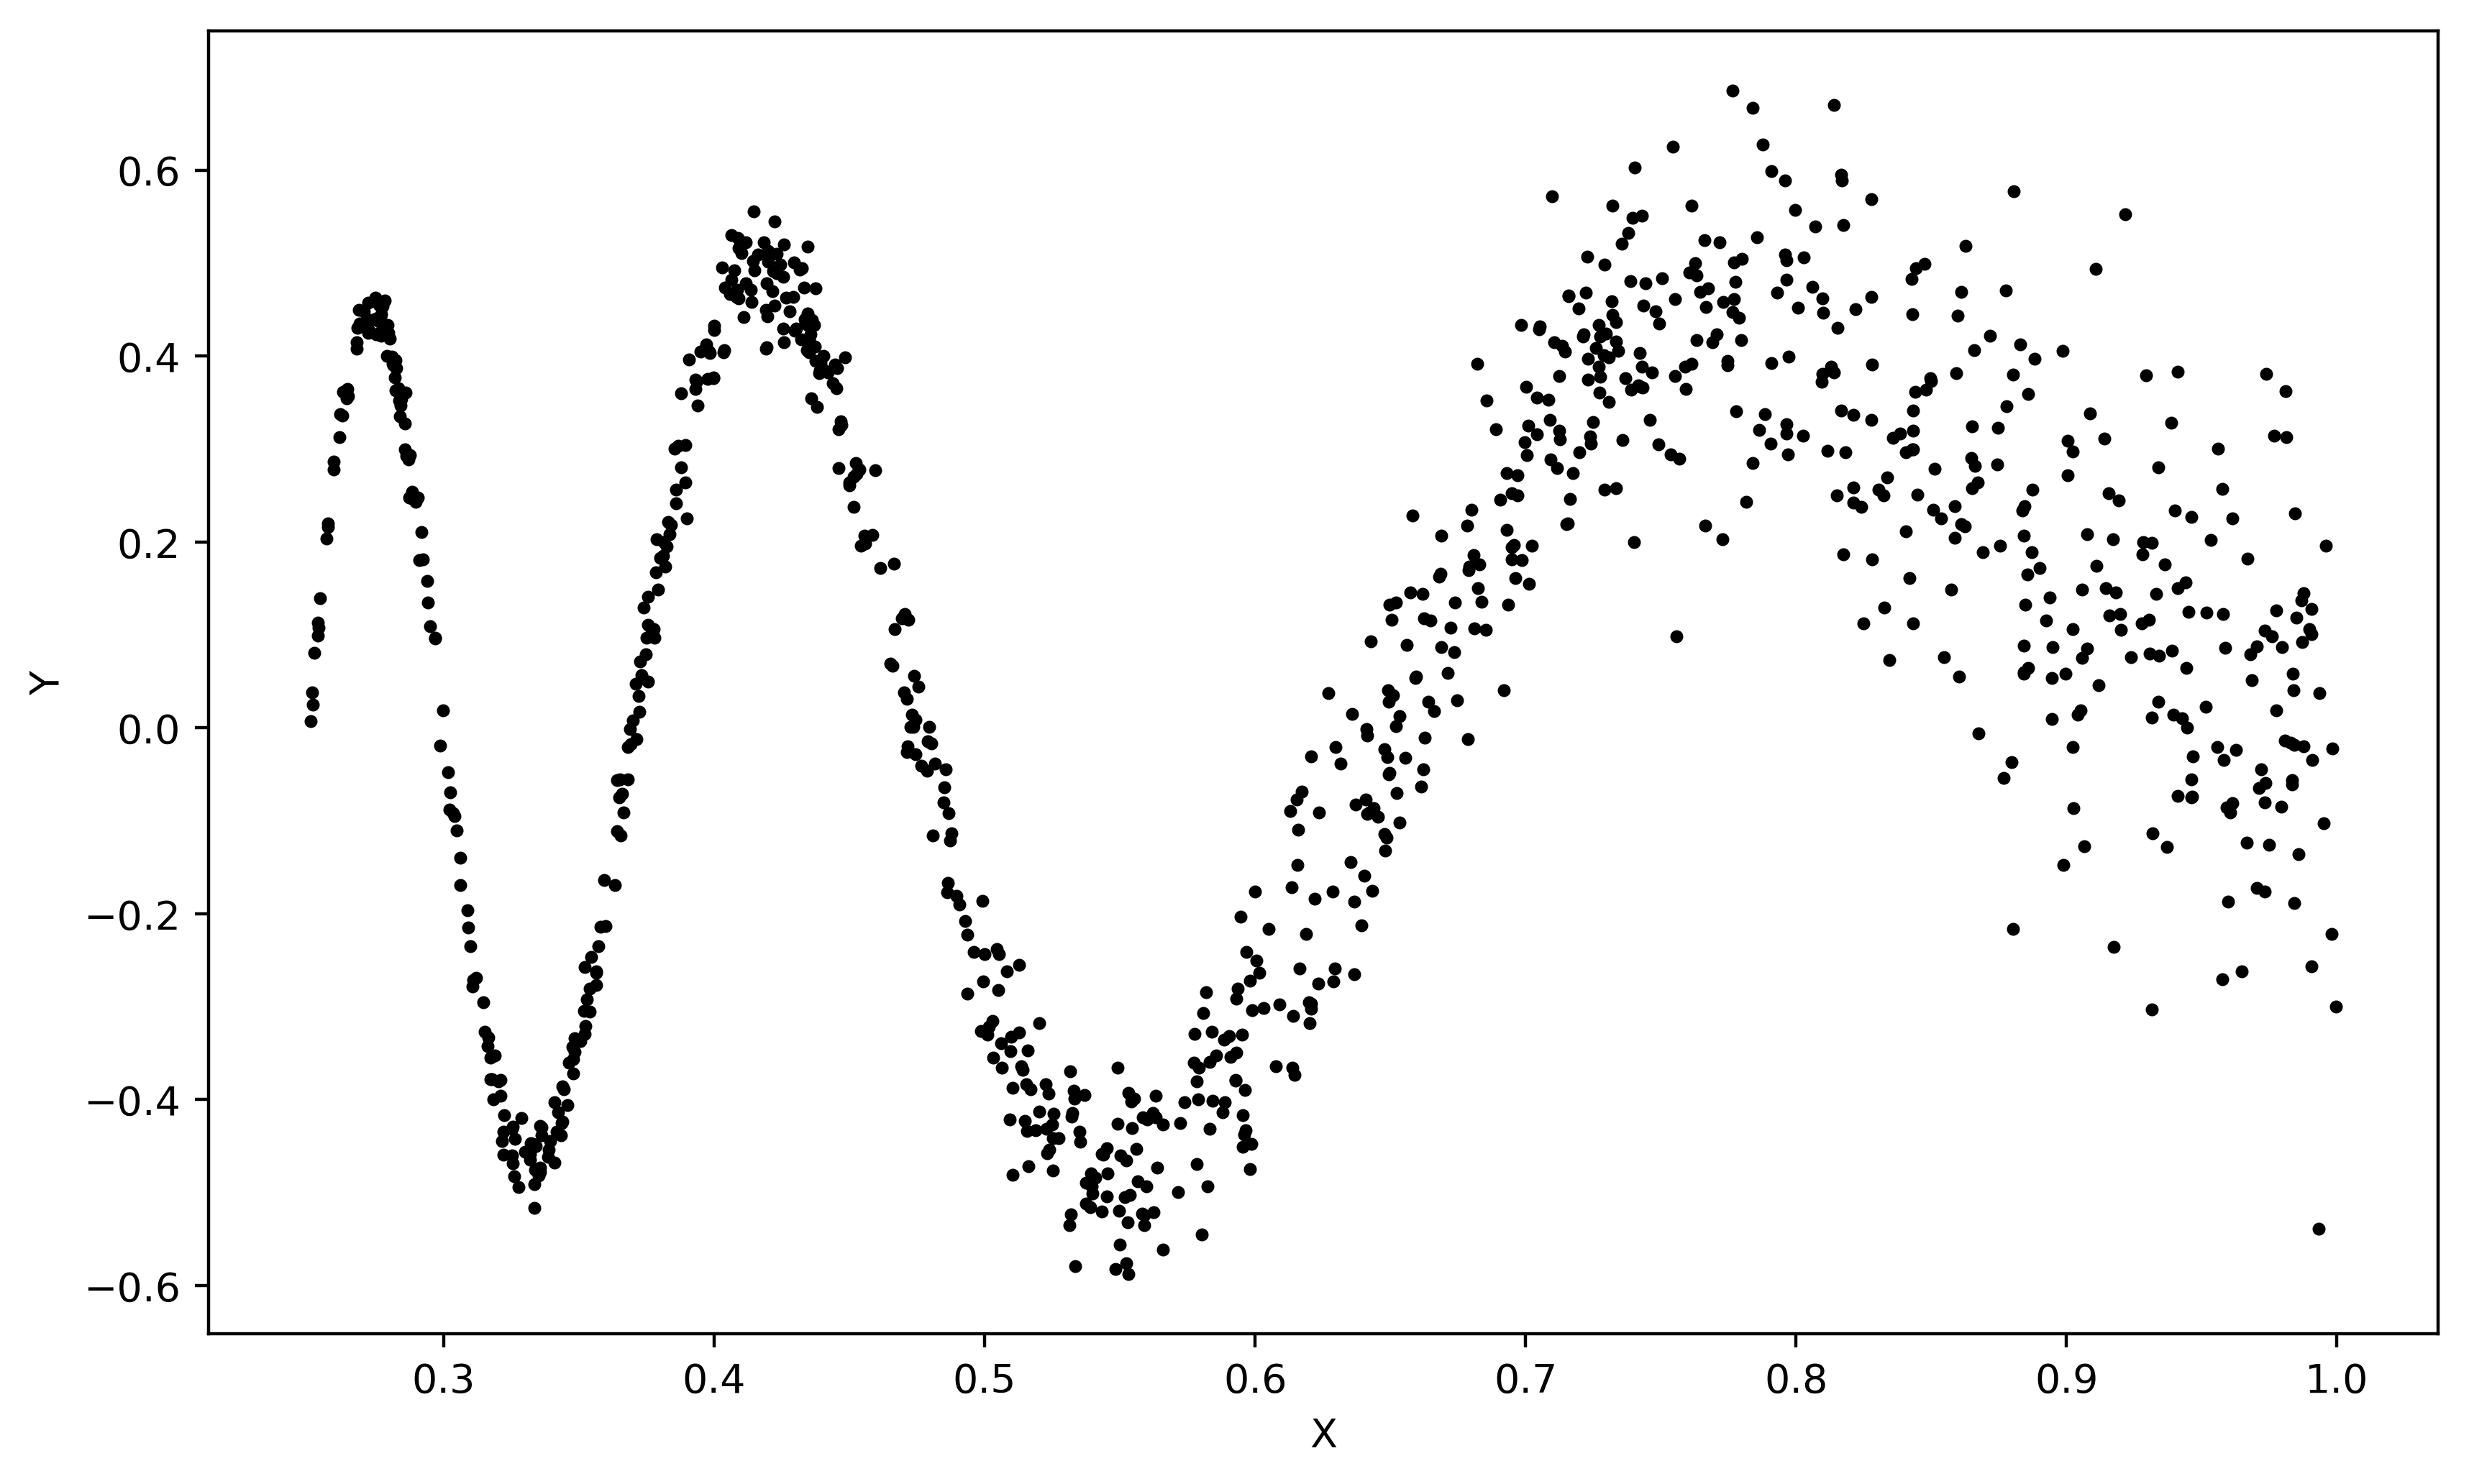
\includegraphics[scale=0.5]{regresionvar}
\end{frame}


\begin{frame}
\frametitle{Estimación de $\sigma^{2}(x)$}

\center
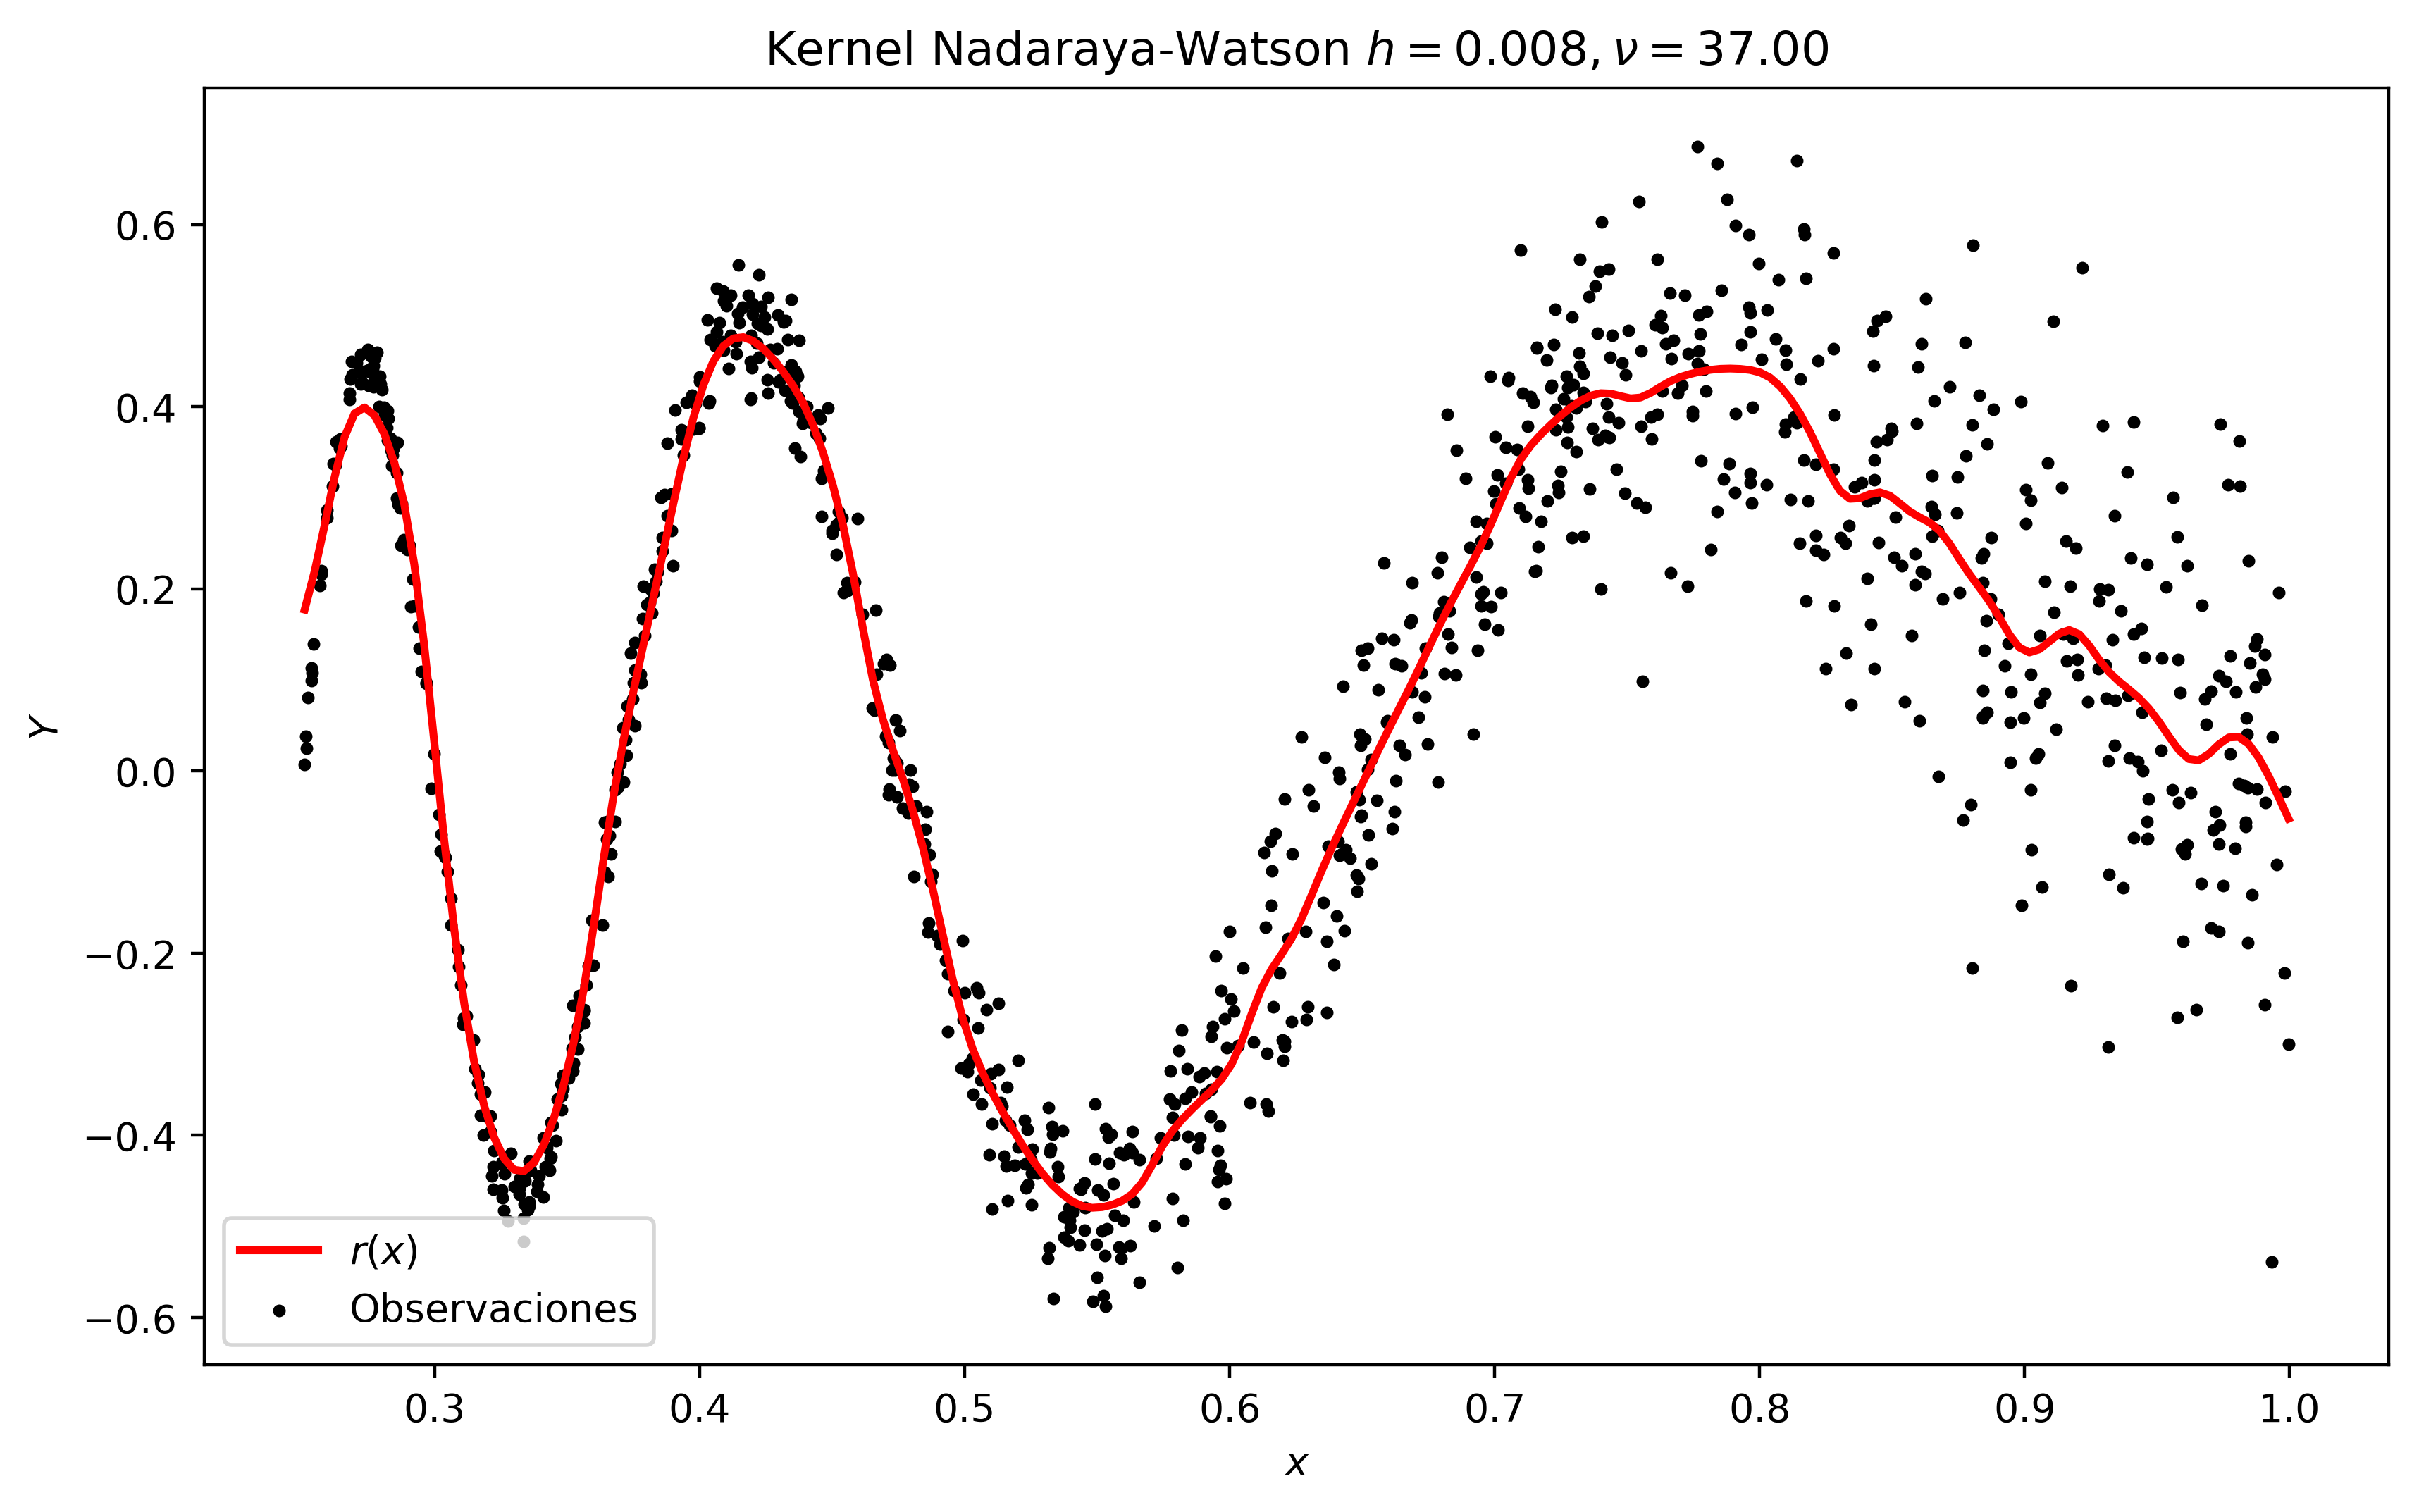
\includegraphics[scale=0.5]{regresionvar2}
\end{frame}


\begin{frame}

\frametitle{Estimación de $\sigma^{2}(x)$}
En este caso podemos asumir que la varianza esta en función de $x$, podemos suponer que 
$$Y_i = r(x_i) + \sigma(x_i)\varepsilon_i$$ 
Con este modelo y teniendo una estimación de $r$, podemos hacer regresión para $\sigma(x)$. Si definimos $Z_i=\log(Y_i-r(x_i))^2$ y $\delta_i=\log\varepsilon_i$ entonces $$Z_i=\log(\sigma^2(x_i))+\delta_i$$
Ahora podemos hacer regresión de $Z_i$ con las $x_i$
\end{frame}

\begin{frame}
\frametitle{Estimación de $\sigma^{2}(x)$}

\center
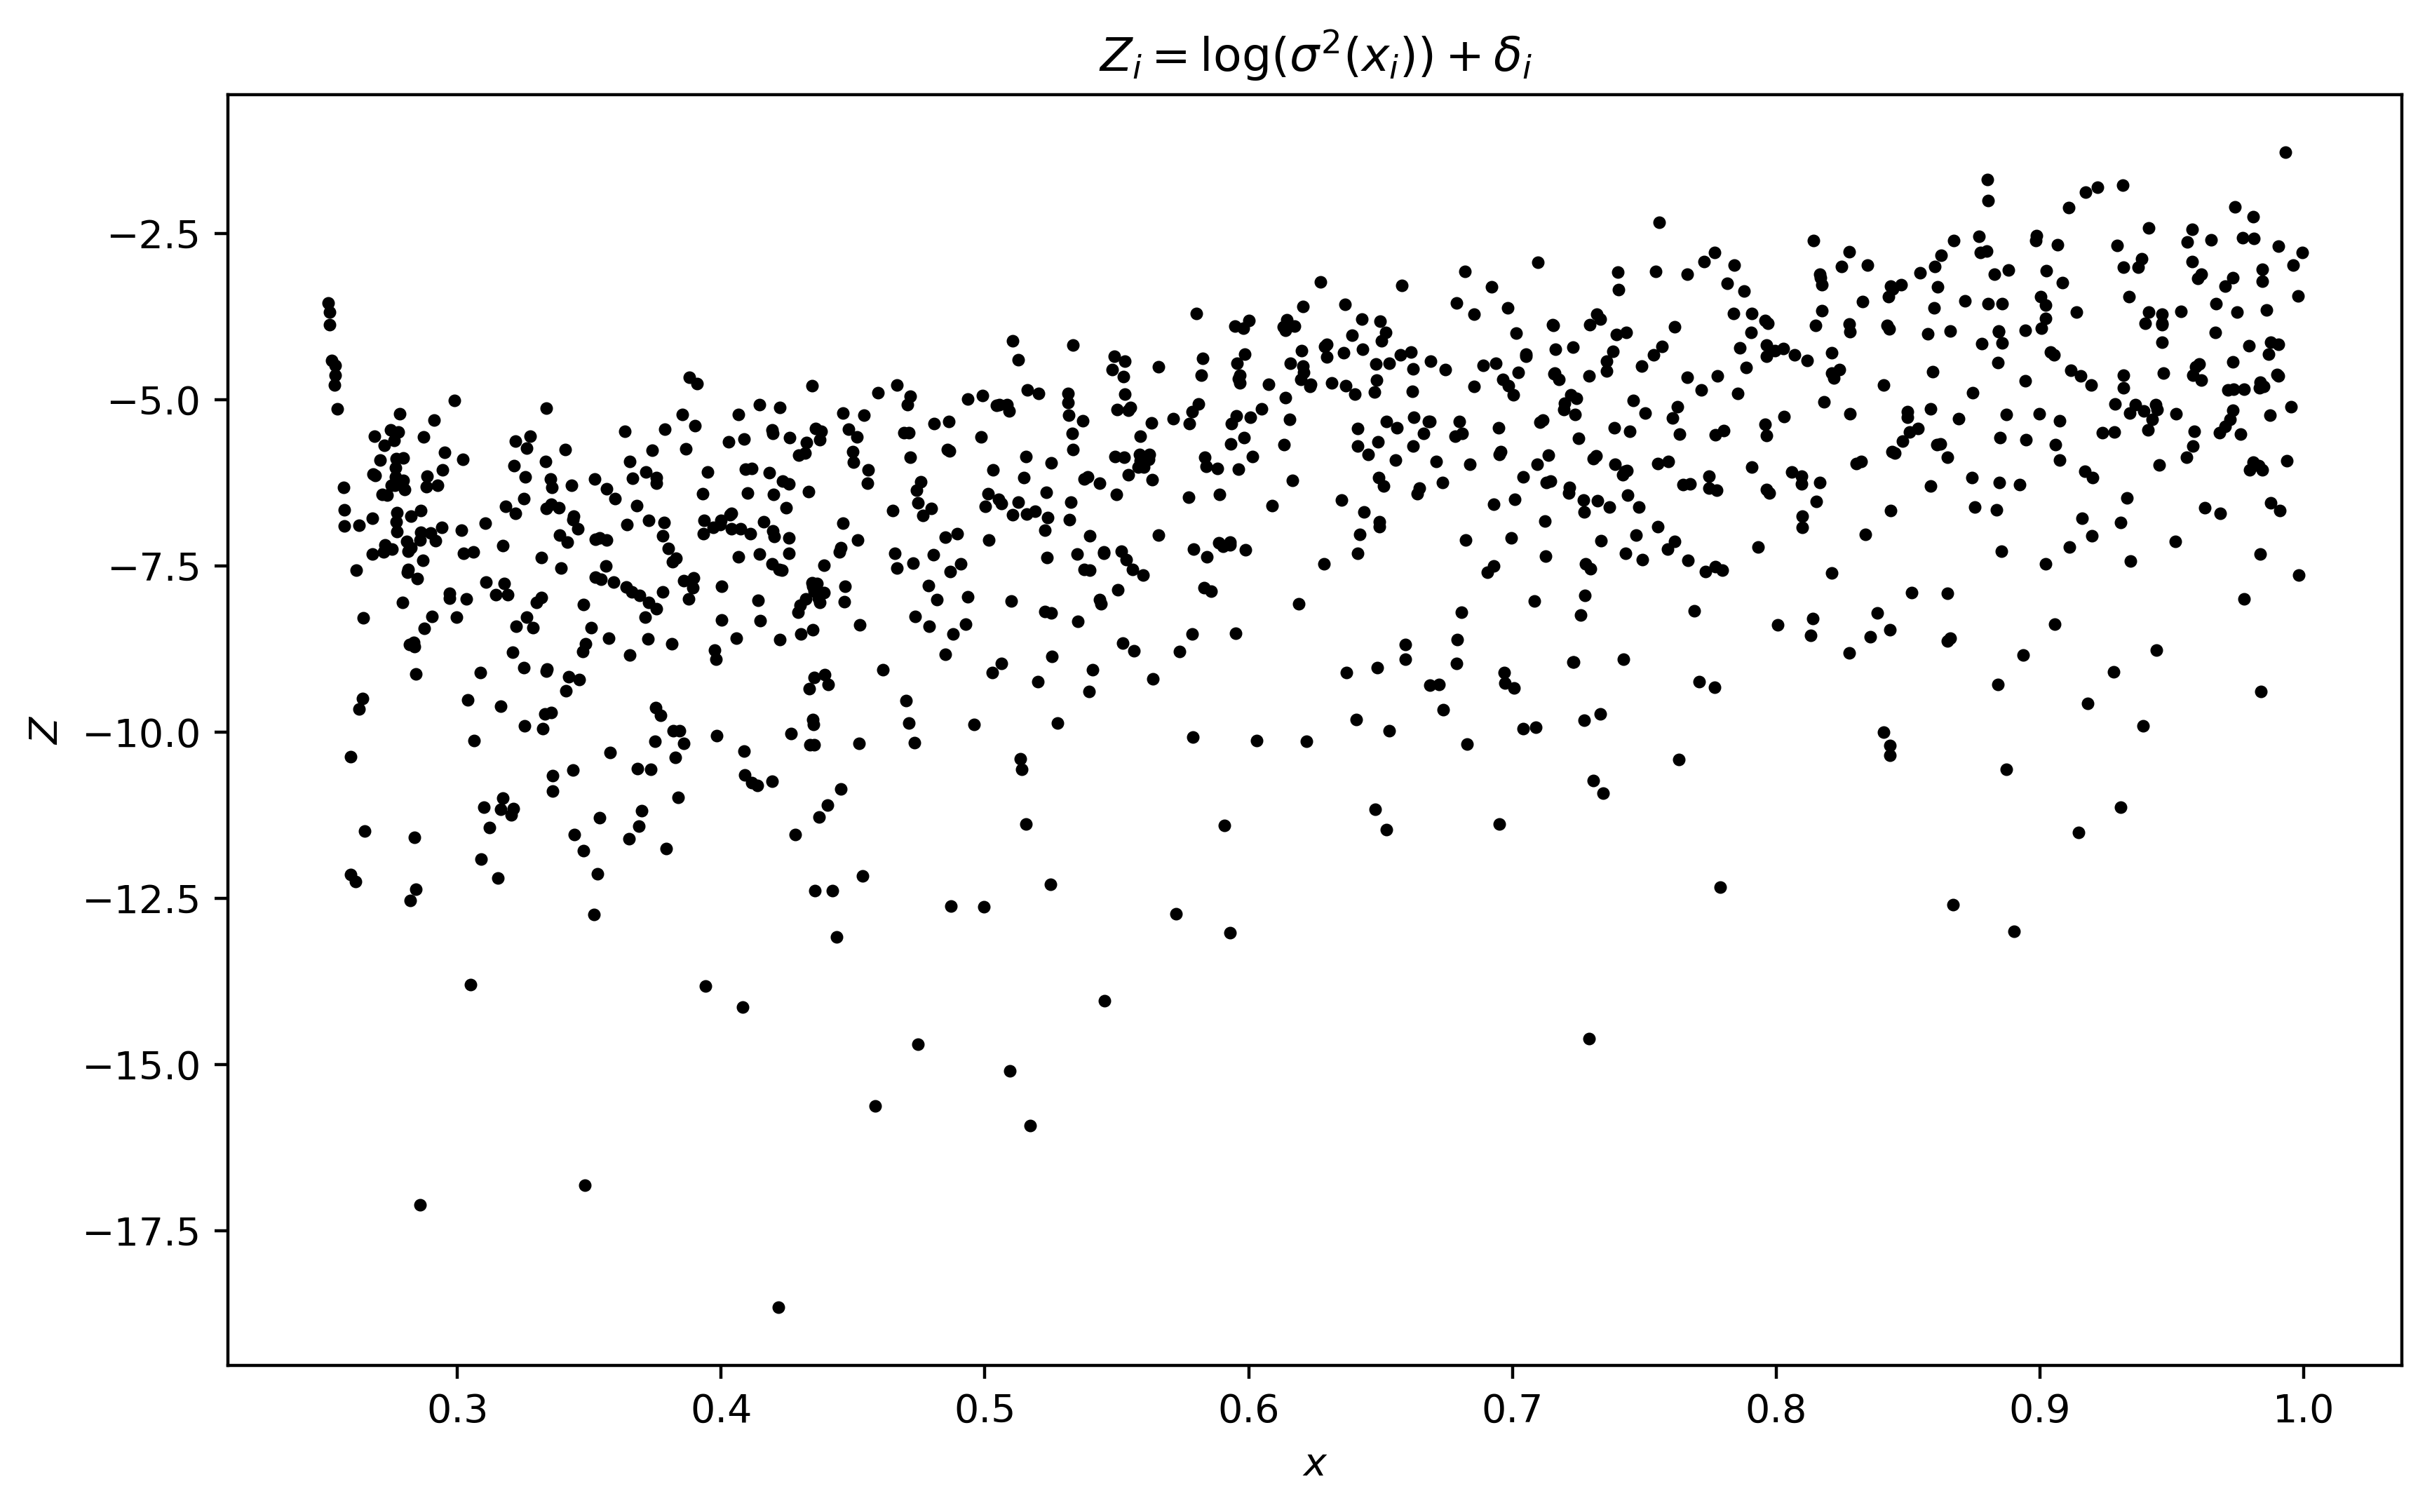
\includegraphics[scale=0.5]{var}
\end{frame}

\begin{frame}
\frametitle{Estimación de $\sigma^{2}(x)$}
\center
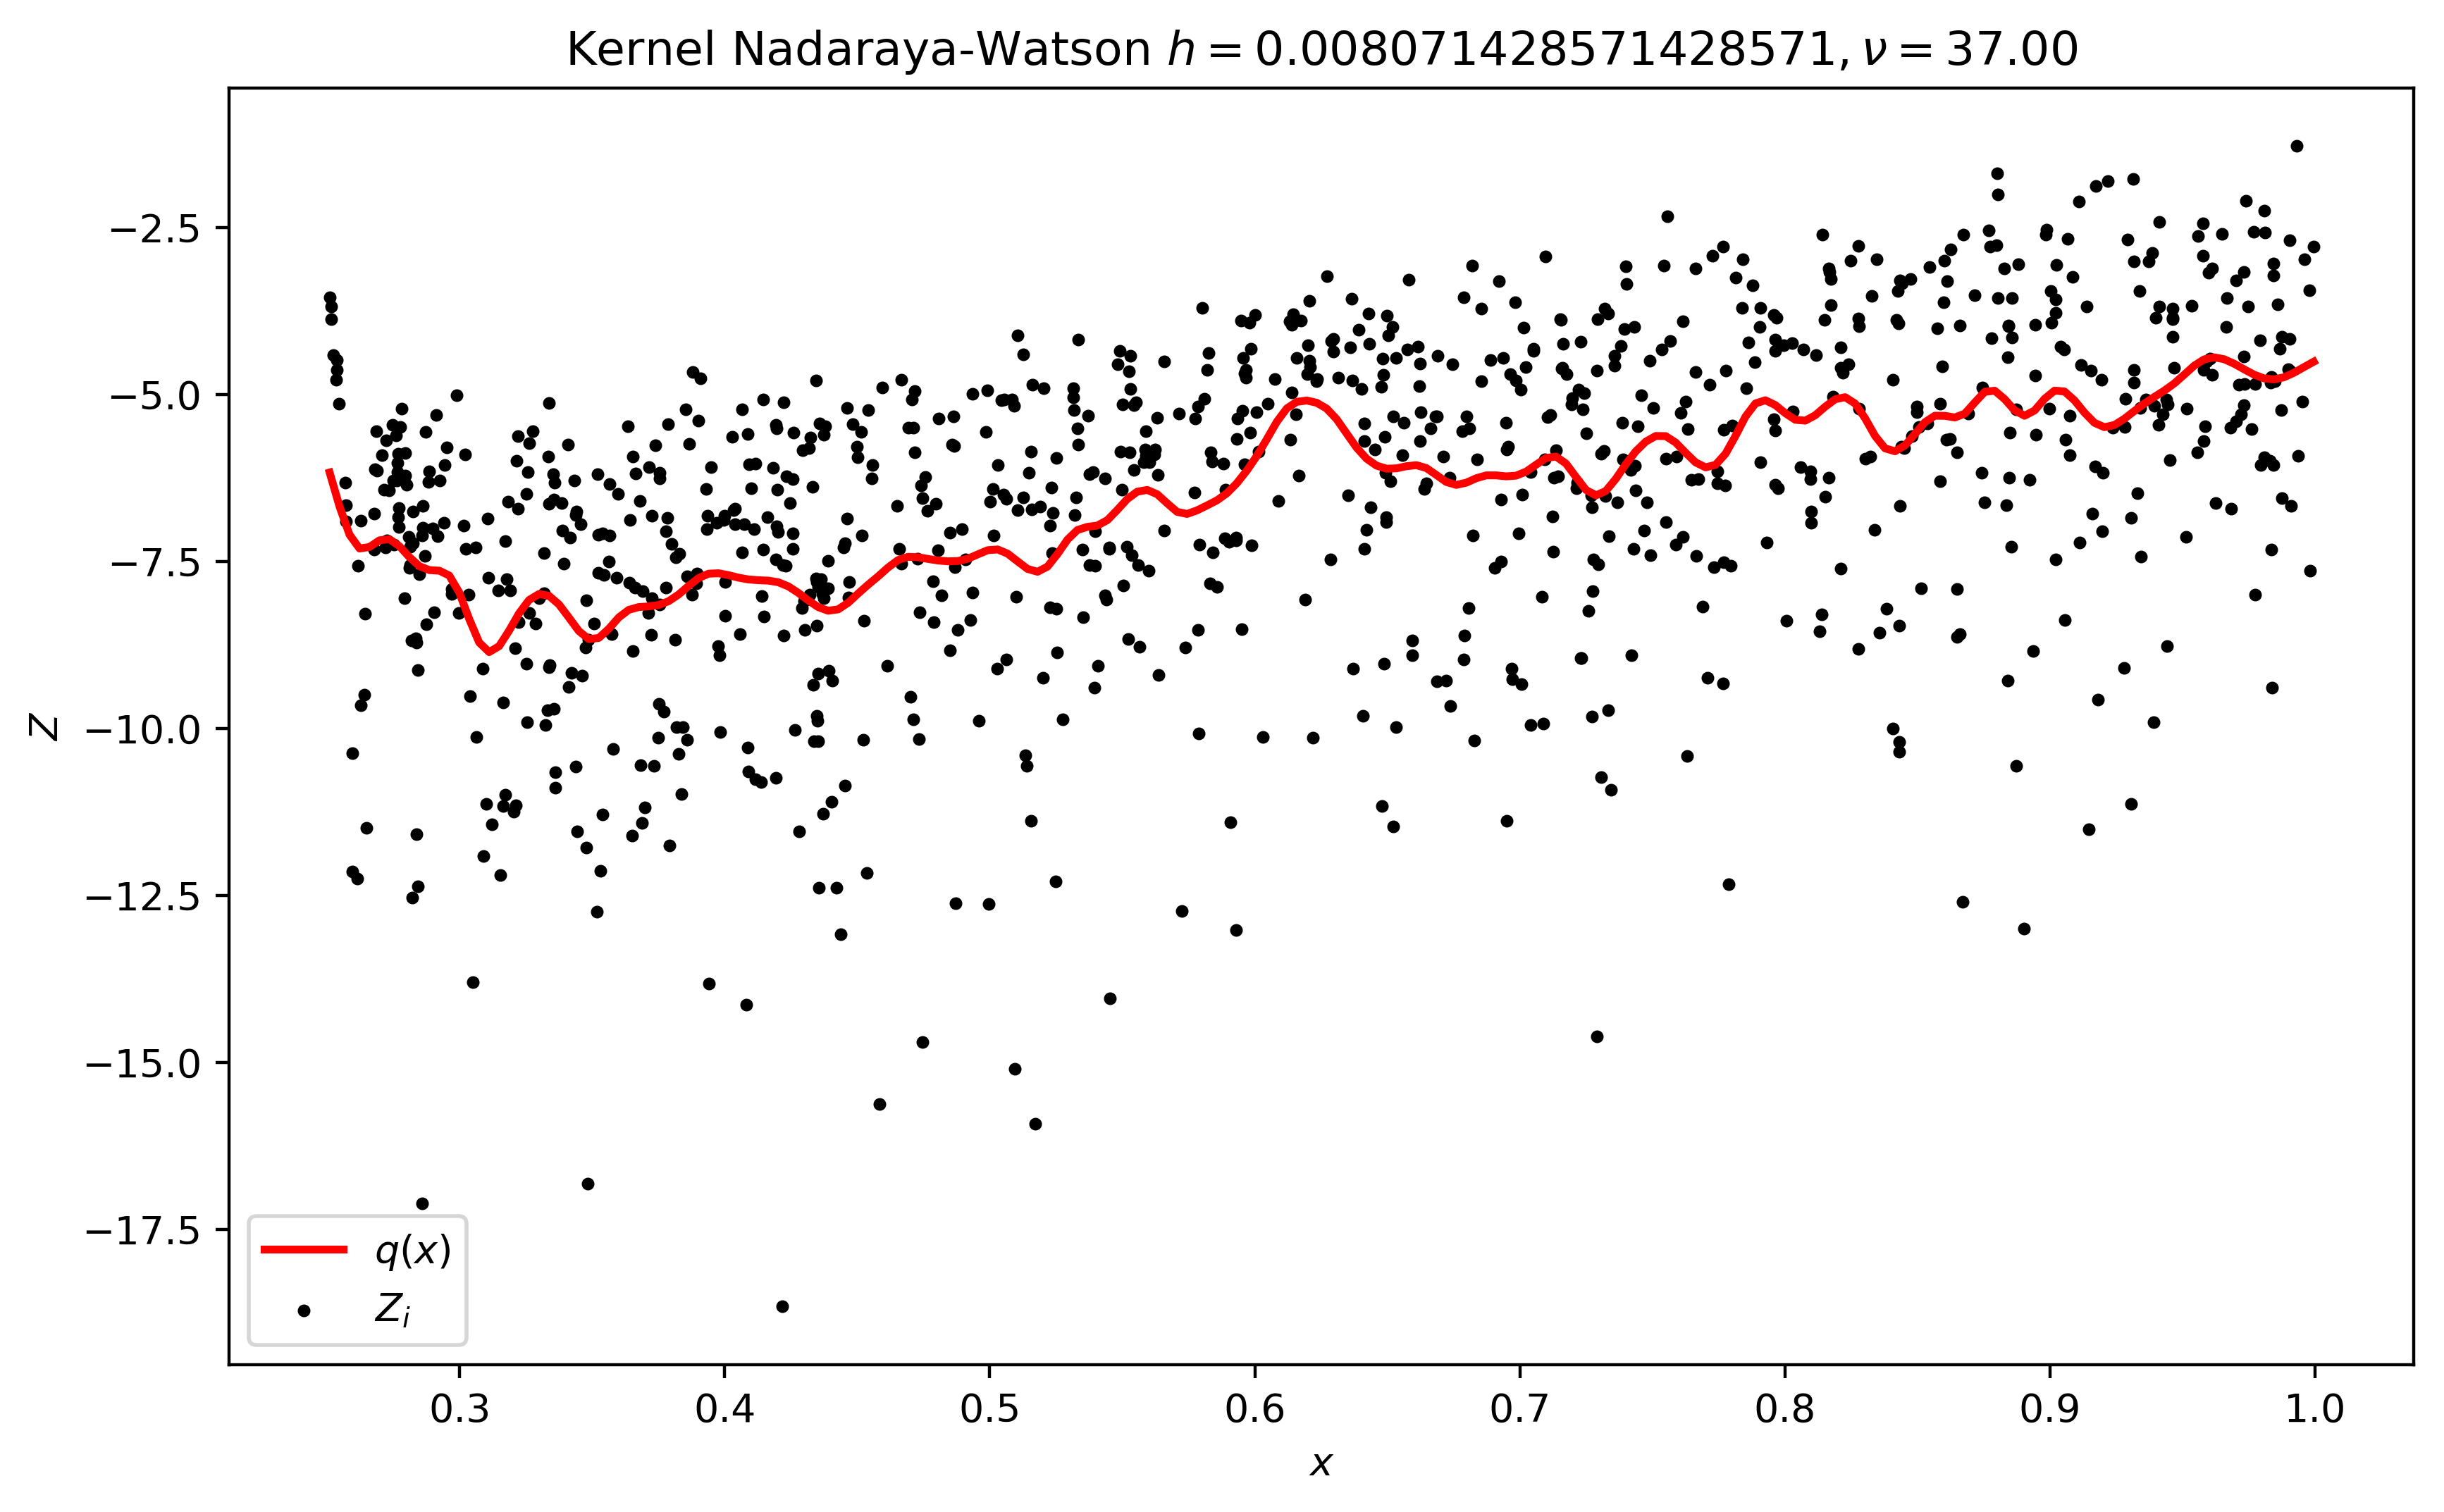
\includegraphics[scale=0.5]{var2}
\end{frame}


\begin{frame}
\frametitle{Estimación de $\sigma^{2}(x)$}
Sin embargo al hacer la regresión y obtener $\hat{q}_n(x)$ solo tenemos que exponenciar ya que $$\sigma^2(x)=e^{q(x)}$$
\end{frame}

\begin{frame}
\frametitle{Estimación de $\sigma^{2}(x)$}
\center
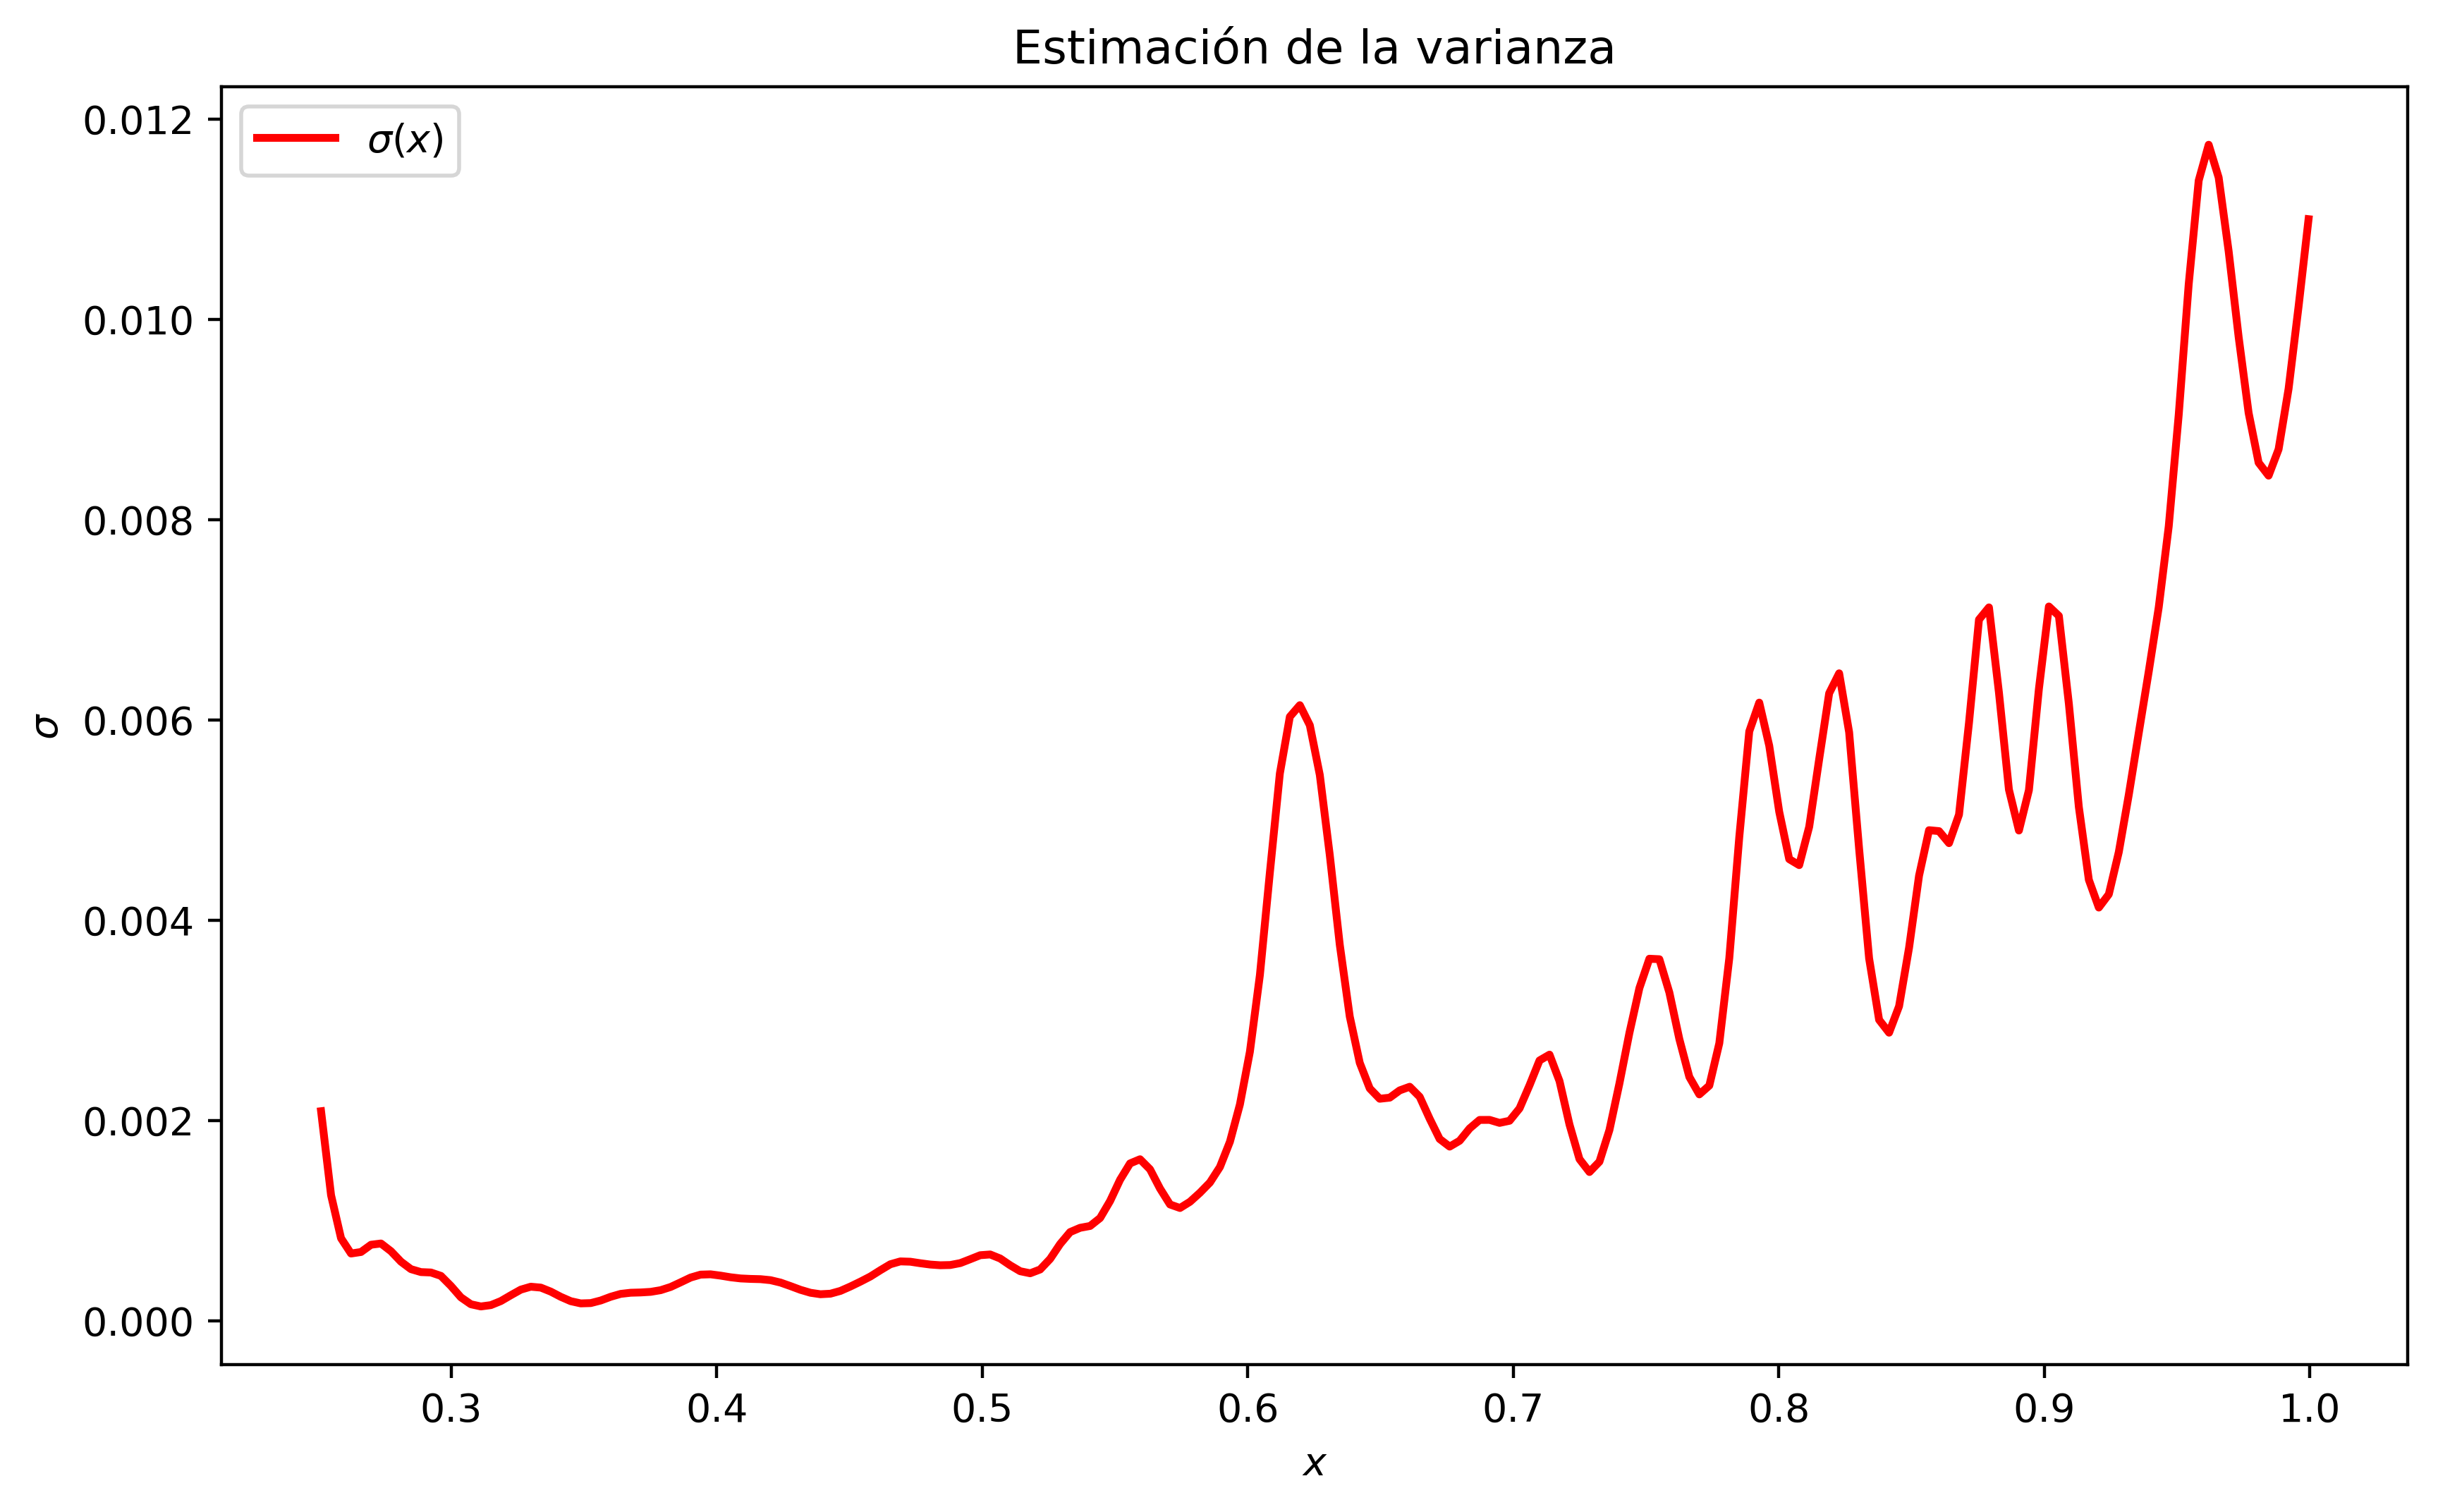
\includegraphics[scale=0.5]{var3}
\end{frame}


\end{document}